\documentclass[runningheads]{llncs}
\usepackage{float}
\usepackage{graphicx}
\usepackage[text={150mm,220mm},centering,nohead]{geometry}
\usepackage{listings}

\usepackage{color}
\definecolor{gray}{rgb}{0.4,0.4,0.4}
\definecolor{darkblue}{rgb}{0.0,0.0,0.6}
\definecolor{cyan}{rgb}{0.0,0.6,0.6}

\lstset{
  basicstyle=\ttfamily,
  columns=fullflexible,
  showstringspaces=false,
  commentstyle=\color{gray}\upshape
}
\lstset{breaklines}
\lstdefinelanguage{XML}
{
  morestring=[b]",
  morestring=[s]{>}{<},
  morecomment=[s]{<?}{?>},
  stringstyle=\color{black},
  identifierstyle=\color{darkblue},
  keywordstyle=\color{cyan},
  morekeywords={xmlns,version,type}% list your attributes here
}
\pagestyle{empty}
\begin{document}
\title{\large{CSCI927 Service-Oriented Software Engineering (Project Report)}}
\author{}
\institute{}
\maketitle
\vspace{-1cm}
%-----------Please Do NOT change the content above.-----------------

%---------------------------------------------------------------------------------------------------------------------------------

%-----------Please write the project information here.---------------

\begin{center}
\Large{\textbf{Online study lounge system based on SOA}} \\ % Please write your project tile in here
\vspace{0.2cm}
\large{\emph{ Group Members (Group 2): Liting Lyu (6603324), Yueyue  He (6603671), Muzhe Peng (6603646), Wangzhihui Mei (6603385)}}\\%Please write names of your group members as well as the group number in here
\vspace{0.3cm}
\end{center}

%-----------Please write the content of your research proposal from here.---------------
\noindent 
\section{The overall work}
At present, the design of the online study lounge system has been completed. The system is designed to help students create a good online learning environment through self-study module, interaction module, question and answer module and personal module. It is based SOA.


%Liting Lyu
Self-study module completes the design of Self-study room service, Attendance service, Learning task service (Must-have) and Taking course service (Good-to-have). Software engineering technology (BPMN, CMMN, DMN, XML, WSC, Flowchart…) are used. This module meets the need of students for self-study, attendance supervision, learning task supervision and sharing courses. The module creates an efficient learning environment for students and make progress with like-minded partners.


%Yueyue  He
The Personal module completes the design of User login service, Password retrieval service, Modification of personal information service, Planning service, Management of network disk and Generation of learning report service. Software engineering technology (BPMN, CMMN, XML, Petri Net, semantic analysis…) are used. This module enables users to properly manage their own information and resources, master their learning progress by generating learning reports, and make adjustments at any time to make learning better.


%Muzhe Peng
Interaction module completes the design of Updates-issue service, Search service, Message-processing service(must-have), Friendlist-viewing service(good-to-have). Software engineering technology (BPMN, CMMN, XML, Petri Net, semantic effect annotation and web service orchestration) are used. This module allows users to interact with others by meaning of sending/replying message, asking/answering questions, issuing/commenting on updates etc. The aim of this module is to help students better study by making communication with those who have the same goals.


%Wangzhihui Mei
Q\&A Module finished the question add/edit/remove/follow and answer add/edit/remove/comment/vote service(must-have services).  Techniques used include BPMN, CMMN, XML, on demand OE, UML, semantical effect annotation. The module can be used to perform FAQ, user can create question and some other one can answer it.
\section{Technical summary}
BPMN, CMMN, DMN, XML, WSC, Flowchart, Petri Net, Semantic effect annotation, Web service orchestration, on demand OE, UML and so on.

%------------Please just change the "project title" and the group members' names in this block-------------------------------
\clearpage
\begin{flushleft}
\huge{\textbf{Appendix}}
\end{flushleft}
\begin{center}
\Large{\textbf{Project Title: CSCI927 Service-Oriented Software Engineering (Project Report) }} \\*[0.1cm]%Please write names of the project title in here
\large{\emph{Group Members (Group 2): Liting Lyu (6603324), Yueyue  He (6603671), Muzhe Peng (6603646), Wangzhihui Mei (6603385)}} %Please write names of your group members as well as the group number in here
\end{center}
%----------------------------------------------------------------------------------------------------------------------------


%-----------Please write the content of your appendix (diagrams, figures, tables, etc) from here.---------------
\section{Supplement the pictures in progress report}
\subsection{Fig. 1. Question Service}
In Question Service, if user encounter some puzzle, he then search question. Then if he find no relative question, he would add question about for the puzzle and follow the question. When new answers are received, user will view the answers. In the other situation, user browse relative qustions and view answers. Then if user find no helpful answers, he will invite some user to answer the question. Else if user find no answers for 10 days, he will edit the question, and follow the question, when new answers are received, he will view the answers. If user find helpful answer, he will vote answer or comment answer and terminate the process.
\subsection{Fig. 2. Answer Service}
The process starts with the process of viewing question or receiving invitation of answering question. Then answerer will add answer to the question. Then when comment messages are received, answerer will reply the dcomment. When answer get ovedr 100 upvoted, answerer will receive award. When answer get over 50 downvoted, the answerer will edit answer.
\subsection{Fig. 3. Q and A Service CMMN Model}
First, the questioner will prepare question idea, the he should edit title and topic for the question, he can optionally edit detail of the question. Then milestone of Problem Added will be entered. Then questioner will seek help, when answers are received, user can vote answer, questioner should adopt answer. Then the milestone of Problem Completed will be entered. The whole process ends.
\subsection{Fig. 4. Message Management}
In the message processing module, the process starts by receiving a message, the type of the message can be various, e.g. friend-adding application, study-room application, application rejection etc. After viewing the message, the user can choose to process the message or not. There are 2 ways of processing, one is to reply the message, the other is to block the sender so that the user will never receive the sender’s message again.
\subsection{Fig. 5. Updates Issue Management}
In the updates management module, the use can issue (1)personal updates and set updates visibility permission(i.e. only a certain group of users are allowed to view this updates). (2)send study-room invitation to invite other users to join the study room. (3)issue question(s) and leave the question to be answered. 
\subsection{Fig. 6. Search Management}
In the search module, the user can search for (1)a related study room. Then he/she will send the request for joining the selected study room, if the administrator passes this application, the user is allowed to join in the study room, otherwise the user will receive an application rejection. (2)a certain user, by clicking the searching result the user can view searched user’s personal information and send application to add him/her as his/her friend, if the searched user passes this application, he/she will be this user’s friend, otherwise the user will receive an application rejection.(3)a related question, the user can view the question, then he/she can answer the question or add the question to favorites or view answerer’s personal information then send message to the answerer.
\subsection{Fig. 7. Reply a Message}
In this CMMN of replying for a message, the user has to understand the content of the message first before editing text for reply, he/she can choose whether add an/some emoji(s) to be more friendly or accurately convey his/her meaning. Only when the user finishes editing the massage can he/she send this message, the case is over if this message is sent successfully.
\subsection{Fig. 8. Login Service}
This figure describes the user login service. If the user has never registered, he/she can choose whether to register or not. If the user chooses to register, he / she should fill in the basic information and bind the account to his / her email or mobile phone. If users do not want to register, they can also browse non user interface. If the user already has an account, he/she can enter the user name and password to log in and enter the app. If the user name or password is filled in incorrectly, an error message will be generated and the user will be notified. If the user forgets his/her password, he/she can choose to retrieve it. There are two ways to get back, one is to use email verification, the other is to use mobile phone verification. After the user obtains the returned verification code, he can reset the password and save it.
\subsection{Fig. 9. Study Plan Service}
This figure describes the learning plan management service. As shown in the figure, if the user wants to add a new plan, she/he can select the "add new" option. After that, fill in the details of the plan and design the expected time. At this time, the countdown will be started, and the user will be reminded when the expected time is reached. Users can also modify existing plans. For example, after selecting the modify option, users can modify the plan content and expected completion time according to their own situation. Users can also delete plans directly.
\subsection{Personal Information Service}
This picture describes the personal information management service.Users can view their own information. If the user want to change her/his information, he/she can choose "Edit information", then change and save her/his information. Here, users can also apply for authentication. There are two types of certification: individual certification and collective certification. Personal certification is school or work certification, while collective certification is applicable to enterprises and institutions. Users who have completed certification can get some benefits,such as more learning resources. After selecting the authentication type, the user should submit the relevant certification materials to complete the authentication.
\subsection{Fig. 10. Learning Report Service CMMN Model}
If the user wants to generate his own learning report, he/she only needs to click "generate report". The system will query the user's self-study times and time in the current month to generate the report.
\subsection{Fig. 11  Self-study Room Service BPMN Model}
First, the self-study room creator creates self-study room. Then, if much information needs to be updated or the creator wants to remove the self-study room, the creator can delete the self-study room. If little information needs to be updated, the creator can update the self-study room. Then, the creator can put the current self-study room online. When a student finds the self-study room, he/she can send an application for joining self-study room. After the self-study room creator receiving the application for joining self-study room, the creator will judge whether to accept the application. If the application is rejected, then a message will be sent to the student and the process of student will end. However, if the application is accepted, the creator will allow the student in the self-study room and then send a message to student. After joining the self-study room, the student may find some problems about the self-study room. If so, the student has rights to report the self-study room to the administrator. When the administrator receives the report, the administrator will put the self-study room offline. And then send an offline message to the self-study room creator. After receiving the offline message, the creator can update or delete the self-study room. And the follow activities are same as activities referred before.
\subsection{Fig. 12. Report the Self-study Room Service CMMN Model}
When the student finds problems, he/she can prepare report. During the student preparing the report, first, he/she will take the evidence. If the student is not sure if the behavior breaks the self-study room management rules, he/she can choose to check self-study room management rules at his/her will. Then, the student can fill in the report. After preparing, a report will be completed as a milestone. And the completed report is the case file. 
\subsection{Fig. 13. Attendance Service BPMN Model}
In the attendance service, the system will send a reminder to remind the student to clock every day. It will be judged regularly whether a student has not clocked in for 7 consecutive days. If the answer is yes, a message to remove the student from the self-study room will be sent out. However, if the answer is no, the student can clock and then time to learn. In the learning process, if a call comes in, this study will end. Otherwise, a statistics report can be displayed at every 23:00.
\subsection{Fig. 14. Learning Task Service BPMN Model}
In the learning task service, it will be judged regularly whether a student has not made plans for 7 consecutive days. If the answer is yes, a message to remove the student from the self-study room will be sent out. However, if the answer is no, the student can make daily plan and then summarize daily learning results. Then, the student can check the progress of learning task.
\section{Add work}

\begin{figure}[H]
		\centering %图片居中
		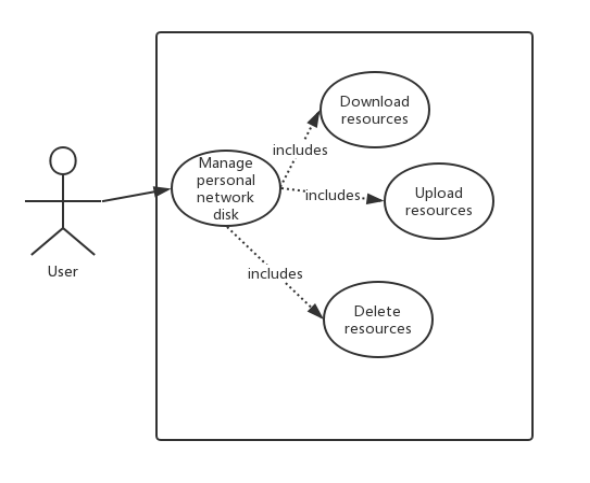
\includegraphics[width=0.8\textwidth]{./figure/Hyy/Usecase} %插入图片,[]中设置图片大小,{}中是图片文件名
		\caption{Usecase diagram of network disk management} %最终文档中希望显示的图片标题
		\label{usecase} %用于文内引用的标签

	\end{figure}
As shown in the figure, users can download the saved resources from their own network disk. You can also upload local resources or delete collected resources.


\begin{figure}[H]
		\centering %图片居中
		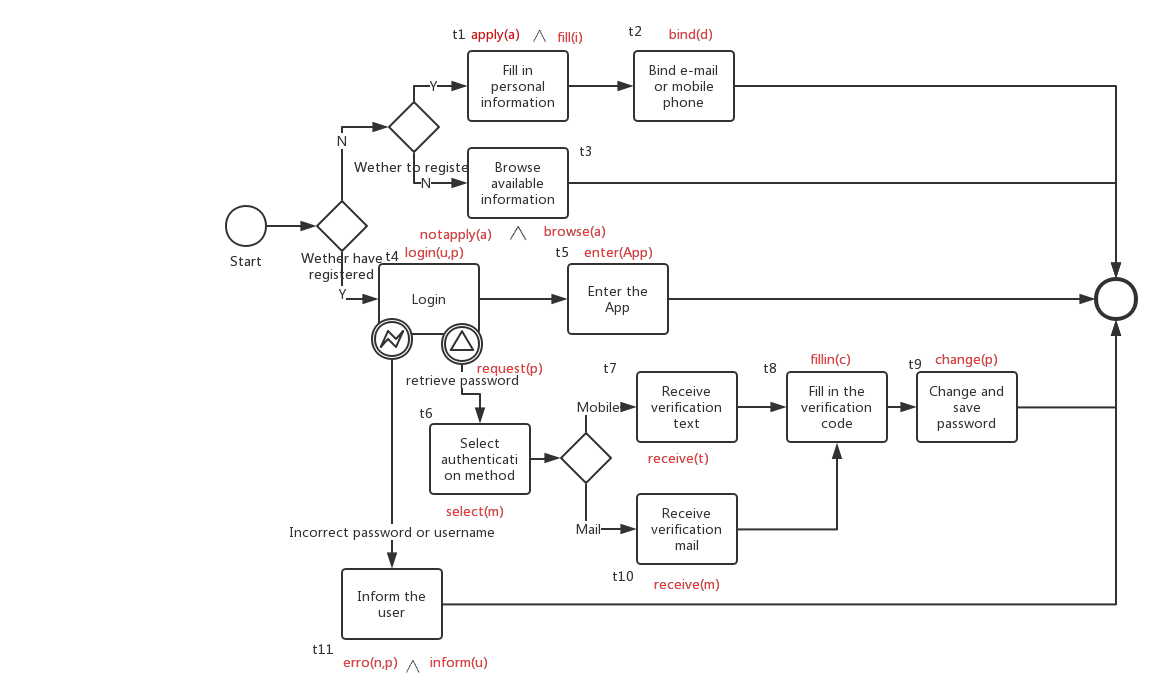
\includegraphics[width=1.0\textwidth]{./figure/Hyy/login} %插入图片,[]中设置图片大小,{}中是图片文件名
		\caption{Semantic analysis of login service} %最终文档中希望显示的图片标题
		\label{login} %用于文内引用的标签
	\end{figure}
Compared with the figure in the progress report, this figure combines the two tasks of filling in the verification code and saving the password. Because in essence, the process of verification is the same whether the verification code is received from mobile phone or email.\\
\\
Relationships between objects:\\
t1:fill(i):fill in user’s personal information i.\\
t2:bind(d):Bind the account to the user's device d.\\
t3:browse(a):Browse non user interface a.\\
t4:login(u,p):Fill in user name u and password p to log in.\\
t5:enter(APP):enter the APP.\\
t6:Select(m):Select password retrieval method m.\\
t7:receive(t):Get verification code from text t.\\
t8:fillin(c):Fill in the verification code c.\\
t9:Change(p):change the password p.\\
t10:receive(m):Get verification code from email m.\\
t11:inform(u):Inform the user u that the user name or password is filled in incorrectly.\\
\\
Cumulative Effect Scenarios:\\
t1:unregistered(u) $\wedge$ apply(a) $\wedge$ fill(i)\\
t2:unregistered(u) $\wedge$ apply(a) $\wedge$ fill(i) $\wedge$ bind(d)\\
t3:unregistered(u) $\wedge$ notapply(a) $\wedge$ browse(a)\\
t4:registered(u) $\wedge$ login(u,p)\\
t5:registered(u) $\wedge$ login(u,p) $\wedge$ enter(APP)\\
t6:registered(u) $\wedge$ login(u,p) $\wedge$ request(p) $\wedge$ select(m)\\
t7:registered(u) $\wedge$ login(u,p) $\wedge$ request(p) $\wedge$ select(M) $\wedge$ receive(t)\\
t8:registered(u) $\wedge$ login(u,p) $\wedge$ request(p) $\wedge$ select(M) $\wedge$ (receive(t) $\vee$ receive(m)) $\wedge$ fillin(c)\\
t9:registered(u) $\wedge$ login(u,p) $\wedge$ request(p) $\wedge$ select(M) $\wedge$ (receive(t) $\vee$ receive(m)) $\wedge$ fillin(c) $\wedge$ change(p)\\
t10:registered(u) $\wedge$ login(u,p) $\wedge$ request(p) $\wedge$ select(M) $\wedge$ receive(m)\\
t11:registered(u) $\wedge$ login(u,p) $\wedge$ error(n,p) $\wedge$ inform(u)\\
\\
t1:Scenario(1):$<$$<$t1$>$,\{$<$t4$>$\}$>$\\
t2:Scenario(1):$<$$<$t1,t2$>$,\{$<$t4$>$\}$>$\\
t3:Scenario(1):$<$$<$t3$>$,\{$<$t4$>$\}$>$\\
t4:Scenario(1):$<$$<$t4$>$,\{$<$t1$>$\}$>$\\
t5:Scenario(1):$<$$<$t4,t5$>$,\{$<$t1$>$\}$>$\\
t6:Scenario(1):$<$$<$t4,t6$>$,\{$<$t1$>$\}$>$\\
t7:Scenario(1):$<$$<$t4,t6,t7$>$,\{$<$t1$>$\}$>$\\
t8:Scenario(1):$<$$<$t4,t6,t7,t8$>$,\{$<$t1$>$\}$>$\\
---Scenario(2):$<$$<$t4,t6,t10,t8$>$,\{$<$t1$>$\}$>$\\
t9:Scenario(1):$<$$<$t4,t6,t7,t8,t9$>$,\{$<$t1$>$\}$>$\\
---Scenario(2):$<$$<$t4,t6,t10,t8,t9$>$,\{$<$t1$>$\}$>$\\
t10:Scenario(1):$<$$<$t4,t6,t10$>$,\{$<$t1$>$\}$>$\\
t11:Scenario(1):$<$$<$t4,t11$>$,\{$<$t1$>$\}$>$\\
\\

\begin{figure}[H]
		\centering %图片居中
		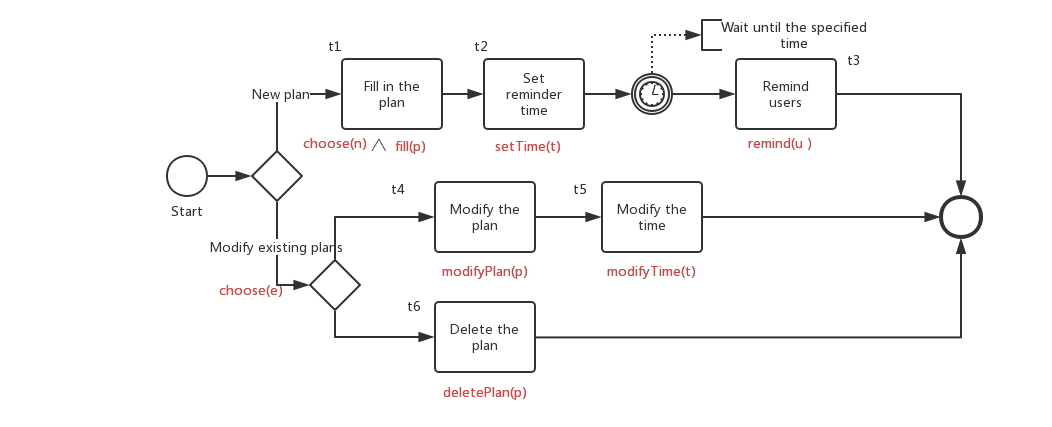
\includegraphics[width=1.0\textwidth]{./figure/Hyy/study} %插入图片,[]中设置图片大小,{}中是图片文件名
		\caption{Semantic analysis of study plan service} %最终文档中希望显示的图片标题
		\label{study} %用于文内引用的标签
	\end{figure}
Compared with the interim report, the figure adds semantic explanation\\
\\
Relationships between objects:\\
t1:fill(p):User can fill in the new plan p.\\
t2:setTime(t):User set the planned completion time t.\\
t3:remind(u):When the expected time is reached, users u will be reminded.\\
t4:modifyPlan(p):Change existing plan p.\\
t5:modifyTime(T):Change the original expected time T.\\
t6:deletePlan(p):Delete original plan p.\\
\\
Cumulative Effect Scenarios:\\
t1:choose(n) $\wedge$ fill(p)\\
t2:choose(n) $\wedge$ fill(p) $\wedge$ setTime(t)\\
t3:choose(n) $\wedge$ fill(p) $\wedge$ setTime(t) $\wedge$ remind(u)\\
t4:choose(n) $\wedge$ modifyPlan(p)\\
t5:choose(n) $\wedge$ modifyPlan(p) $\wedge$ modifyTime(T)\\
t6:choose(n) $\wedge$ deletePlan(p)\\
\\
t1:Scenario(1):$<$$<$t1$>$,\{$<$t4$>$\}$>$\\
t2:Scenario(1):$<$$<$t1,t2$>$,\{$<$t4$>$\}$>$\\
t3:Scenario(1):$<$$<$t1,t2,t3$>$,\{$<$t4$>$\}$>$\\
t4:Scenario(1):$<$$<$t4$>$,\{$<$t1$>$\}$>$\\
t5:Scenario(1):$<$$<$t4,t5$>$,\{$<$t1$>$\}$>$\\
t6:Scenario(1):$<$$<$t6$>$,\{$<$t1$>$\}$>$\\
\\
\begin{figure}[H]
		\centering %图片居中
		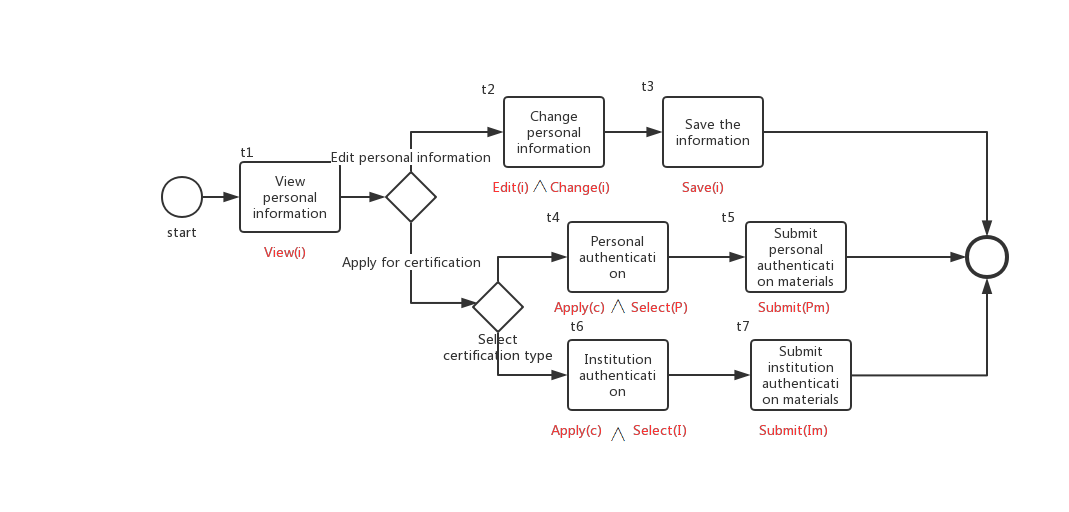
\includegraphics[width=1.0\textwidth]{./figure/Hyy/gg} %插入图片,[]中设置图片大小,{}中是图片文件名
		\caption{Semantic analysis of personal information service} %最终文档中希望显示的图片标题
		\label{study} %用于文内引用的标签
	\end{figure}
Compared with the interim report, the figure adds semantic explanation\\
\\
Relationships between objects:\\
t1:View(i):View user’s personal information i.\\
t2:Change(i):Change user’s personal information i.\\
t3:Save(i):Save changed information i.\\
t4:Select(P):Choose personal authentication method P.\\
t5:Submit(Pm):Submit personal authentication materials Pm.\\
t6:Select(I):Select collective certification method I.\\
t7:Submit(Im):Submit institution authentication materials Im.\\
\\
Cumulative Effect Scenarios:\\
t1:View(i)\\
t2:View(i) $\wedge$ Edit(i) $\wedge$ Change(i)\\
t3:View(i) $\wedge$ Edit(i) $\wedge$ Change(i) $\wedge$ Save(i)\\
t4:View(i) $\wedge$ Apply(c) $\wedge$ Select(P)\\
t5:View(i) $\wedge$ Apply(c) $\wedge$ Select(P) $\wedge$ Submit(Pm)\\
t6:View(i) $\wedge$ Apply(c) $\wedge$ Select(I)\\
t7:View(i) $\wedge$ Apply(c) $\wedge$ Select(I) $\wedge$ Submit(Im)\\
\\
t2:Scenario(1):$<$$<$t1,t2$>$,\{$<$t1,t4$>$\}$>$\\
t3:Scenario(1):$<$$<$t1,t2,t3$>$,\{$<$t1,t4$>$\}$>$\\
t4:Scenario(1):$<$$<$t1,t4$>$,\{$<$t1,t2$>$\}$>$\\
t5:Scenario(1):$<$$<$t1,t4,t5$>$,\{$<$t1,t2$>$\}$>$\\
t6:Scenario(1):$<$$<$t1,t6$>$,\{$<$t1,t2$>$\}$>$\\
t7:Scenario(1):$<$$<$t1,t6,t7$>$,\{$<$t1,t2$>$\}$>$\\
\\
List of states:\\
P1:User;Ready to send request\\
P2:User;Waiting for verification code\\
P3:User;Received verification code\\
P4:User;Modification completed\\
P5:Sever;Waiting for a request\\
P6:Sever;Receive a request\\
P7:Sever;Waiting for material modification\\
P8:Sever;Complete this service\\
\\
t1:User;Send request\\
t2:User;Receive verification code\\
t3:User;Change Password\\
t4:Sever;Acceptance request\\
t5:Sever;Send verification code\\
t6:Sever;Accept and save new password\\
t7:Sever;End process\\

\begin{figure}[H]
		\centering %图片居中
		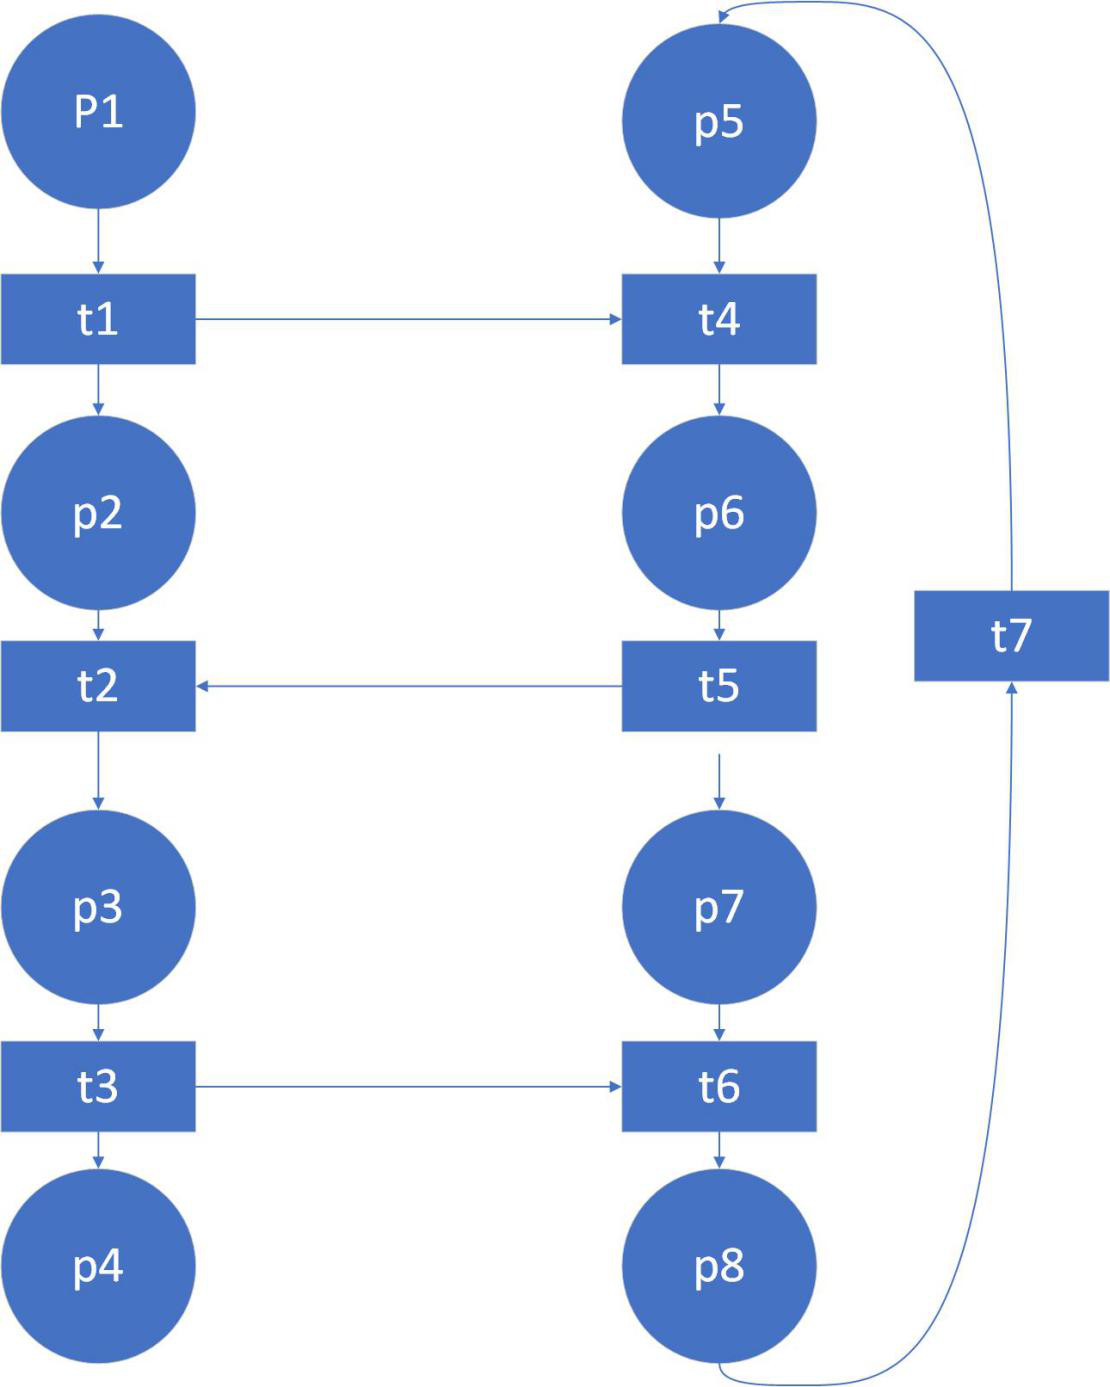
\includegraphics[width=0.5\textwidth]{./figure/Hyy/petri} %插入图片,[]中设置图片大小,{}中是图片文件名
		\caption{Petri Net of Retrieve password service} %最终文档中希望显示的图片标题
		\label{petri} %用于文内引用的标签
	\end{figure}
This figure describes the password retrieval service in the user login service. As shown in the figure, when the server is idle, if it receives the password retrieval request from the client, it will send the verification code to the client. After sending, the server will change to the waiting state, waiting for the password change response from the client. After receiving the new password from the client, the server will save it and complete the process, and then change to idle state, waiting for the new request.

\begin{figure}[H]
		\centering %图片居中
		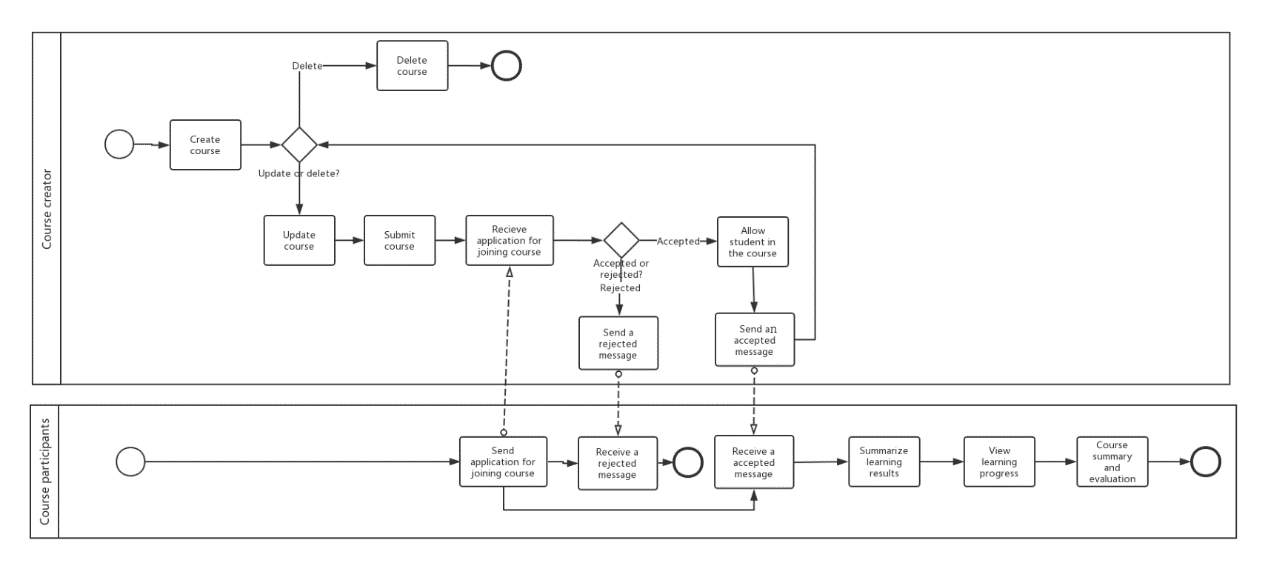
\includegraphics[width=1.0\textwidth]{./figure/LLT/BPMN} %插入图片,[]中设置图片大小,{}中是图片文件名
		\caption{Taking course Service BPMN Model} %最终文档中希望显示的图片标题
		\label{bpmn} %用于文内引用的标签
	\end{figure}
First, the course creator creates course. Then, if much information needs to be updated or the creator wants to remove the course, the creator can delete the course. If little information needs to be updated, the creator can update the course. Then, the creator can submit the course. When a student finds the course, he/she can send an application for joining course. After the course creator receiving the application for joining the course, the creator will judge whether to accept the application. If the application is rejected, then a message will be sent to the student and the process of student will end. However, if the application is accepted, the creator will allow the student in the course and then send a message to the student. After receiving the accepted message, the student can summarize learning results. And then view learning process. And then summarize and evaluate the course. Then the process of student will end. For the course creator, after sending an accepted message, he/she can update or delete the course. And the follow activities are same as activities referred before.
\begin{figure}[H]
		\centering %图片居中
		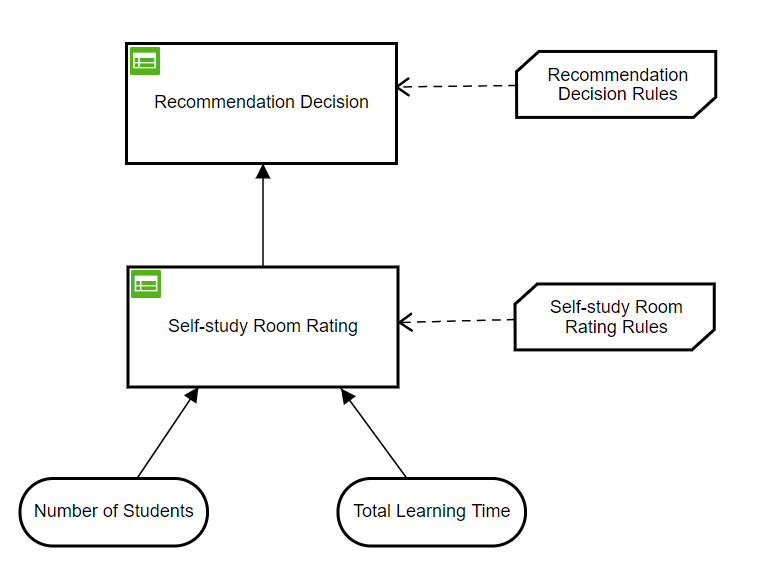
\includegraphics[width=1.0\textwidth]{./figure/LLT/Decision} %插入图片,[]中设置图片大小,{}中是图片文件名
		\caption{Decision Requirements of Self-study Room Rating and Recommendation DMN Model} %最终文档中希望显示的图片标题
		\label{3} %用于文内引用的标签
	\end{figure}
\begin{figure}[H]
		\centering %图片居中
		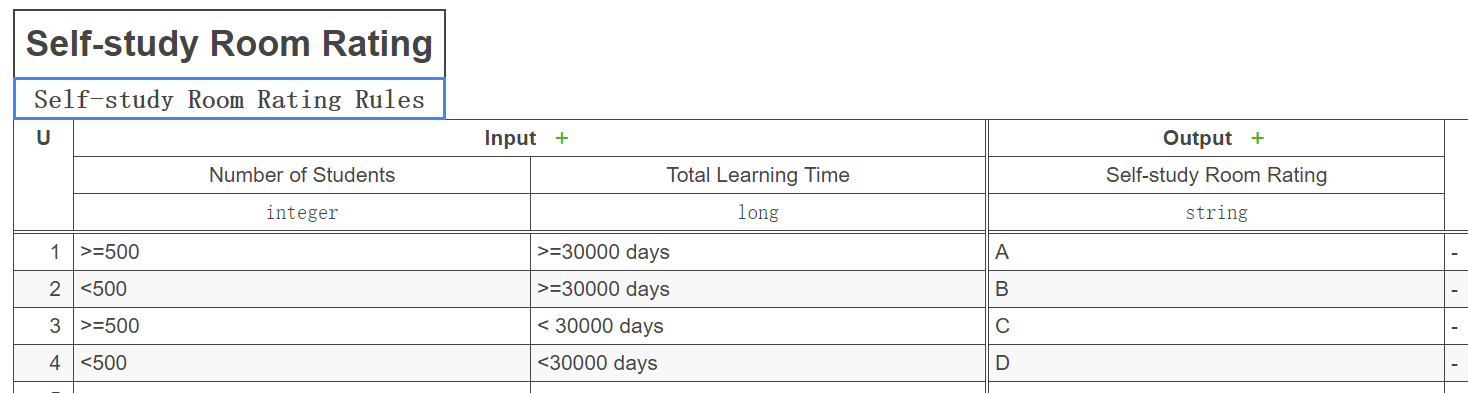
\includegraphics[width=1.0\textwidth]{./figure/LLT/logic} %插入图片,[]中设置图片大小,{}中是图片文件名
		\caption{Decision Logic of Self-study Room Rating and Recommendation DMN Model for Rating Rules} %最终文档中希望显示的图片标题
		\label{2} %用于文内引用的标签
	\end{figure}
\begin{figure}[H]
		\centering %图片居中
		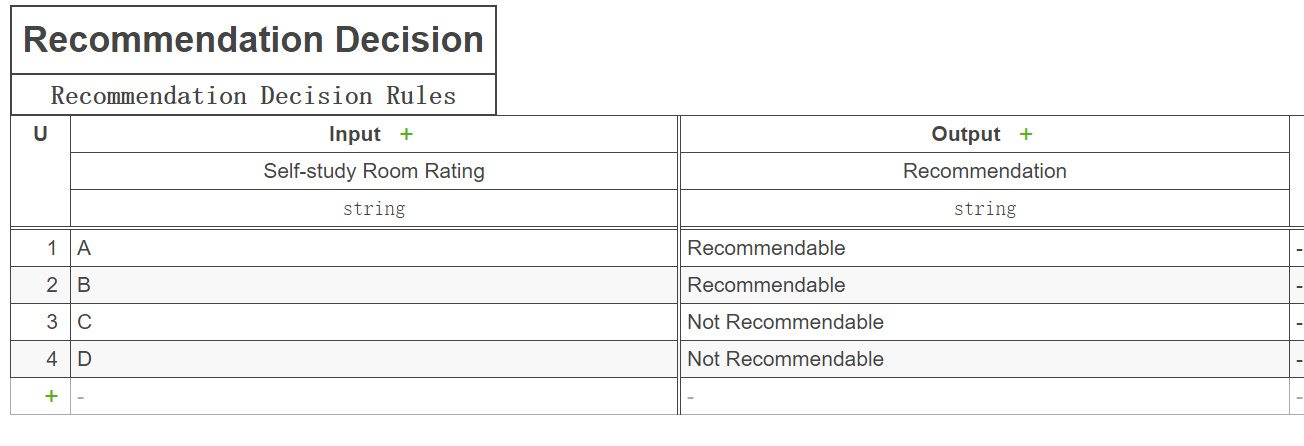
\includegraphics[width=1.0\textwidth]{./figure/LLT/logicw} %插入图片,[]中设置图片大小,{}中是图片文件名
		\caption{Decision Logic of Self-study Room Rating and Recommendation DMN Model for Recommendation Decision Rules} %最终文档中希望显示的图片标题
		\label{1} %用于文内引用的标签
	\end{figure}
The self-study room rating depends on number of students and total learning time. If the number of students is not less than 500 and total learning time is not less than 30000 days, then the self-study room will be rated A. If the number of students is less than 500 and total learning time is not less than 30000 days, then the self-study room will be rated B. If the number of students is not less than 500 and total learning time is less than 30000 days, then the self-study room will be rated C. If the number of students is less than 500 and total learning time is less than 30000 days, then the self-study room will be rated D.

The recommendation decision depends on self-study room rating. If the self-study room is rated A or B, the self-study room will be recommendable. If the self-study room is rated C or D, the self-study room will be not recommendable.
\begin{figure}[H]
		\centering %图片居中
		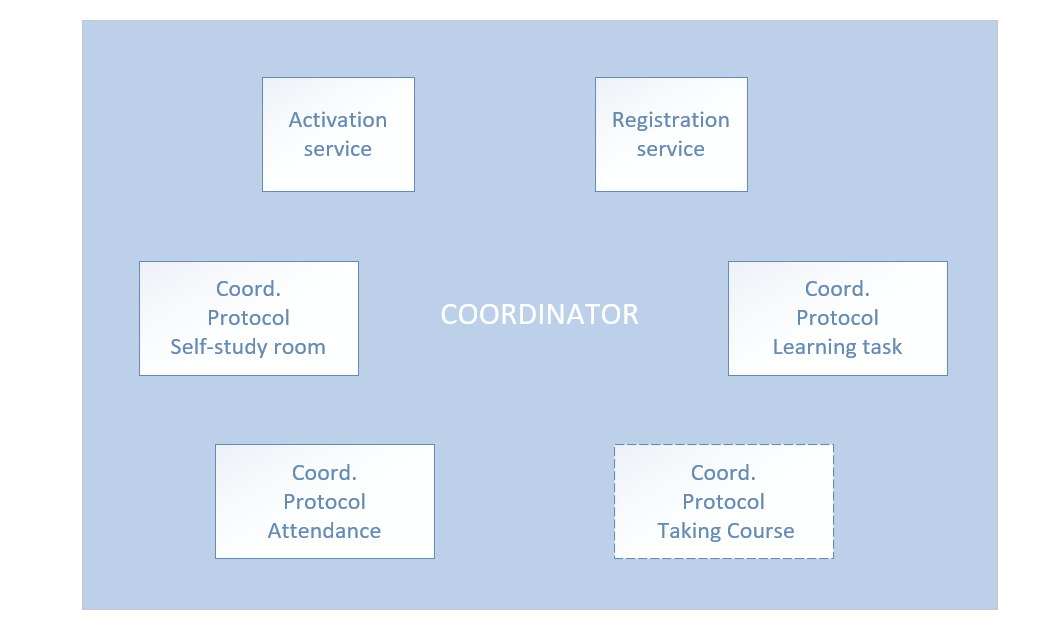
\includegraphics[width=1.0\textwidth]{./figure/LLT/WSC} %插入图片,[]中设置图片大小,{}中是图片文件名
		\caption{Self-study module WS-C Model} %最终文档中希望显示的图片标题
		\label{wsc} %用于文内引用的标签
	\end{figure}
The coordinator for self-study module is consist of activation service, registration service, coordination protocol self-study room, coordination protocol learning task, coordination protocol attendance and coordination protocol taking courses. The activation service is used to start a coordination protocol. The registration service is used to register for a coordination protocol. Coordination protocol self-study room, coordination protocol learning task, coordination protocol attendance and coordination protocol taking courses are used to operate coordination protocol. And they can link with each other under some condition.\\
\begin{figure}[H]
		\centering %图片居中
		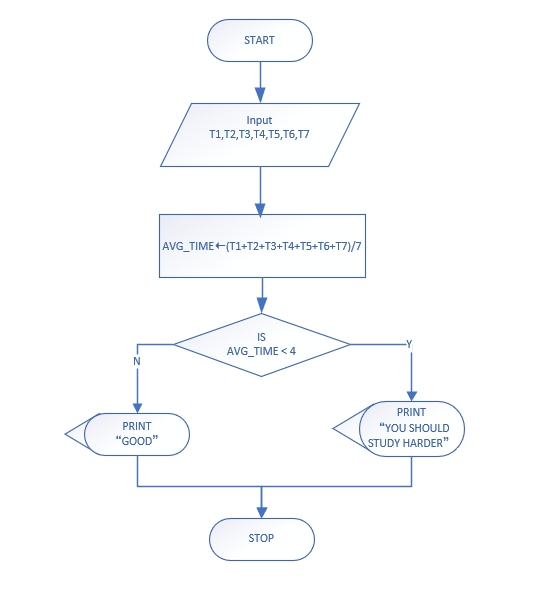
\includegraphics[width=1.0\textwidth]{./figure/LLT/flow} %插入图片,[]中设置图片大小,{}中是图片文件名
		\caption{Reminder of study time Flowchart} %最终文档中希望显示的图片标题
		\label{flow} %用于文内引用的标签
	\end{figure}
Calculate the average time that a student spent on learning in a week. Study time in everyday is represented as T1,T2,T3,T4,T5,T6,T7. If the average<4, print “You should work harder”. Otherwise, print “Good”.

\begin{figure}[H]
		\centering %图片居中
		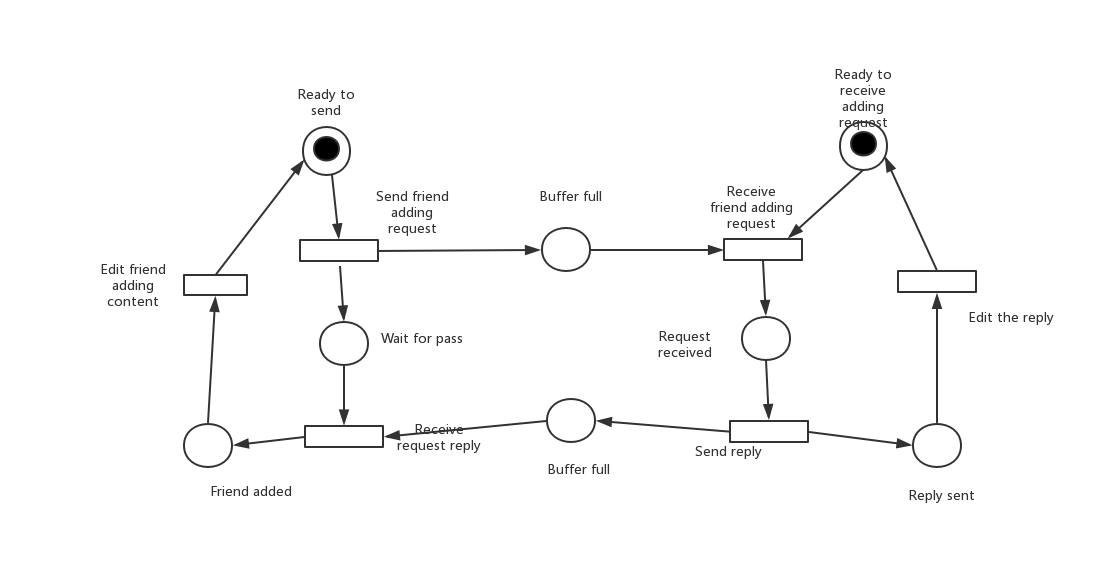
\includegraphics[width=1.0\textwidth]{./figure/PMZ/pe} %插入图片,[]中设置图片大小,{}中是图片文件名
		\caption{Petri Net of Message Reply} %最终文档中希望显示的图片标题
		\label{pe} %用于文内引用的标签
	\end{figure}
At the very beginning, there are 2 users, one is to send friend adding request, the other is to receive friend adding request, there is a token in each of them. Once the sender sent the request, his/her state turns into the state of waiting for the request pass, once the receiver receives request, he/she will give some reply to inform the sender. Only when the sender receive the request reply can he/she add friend successfully.
\begin{figure}[H]
		\centering %图片居中
		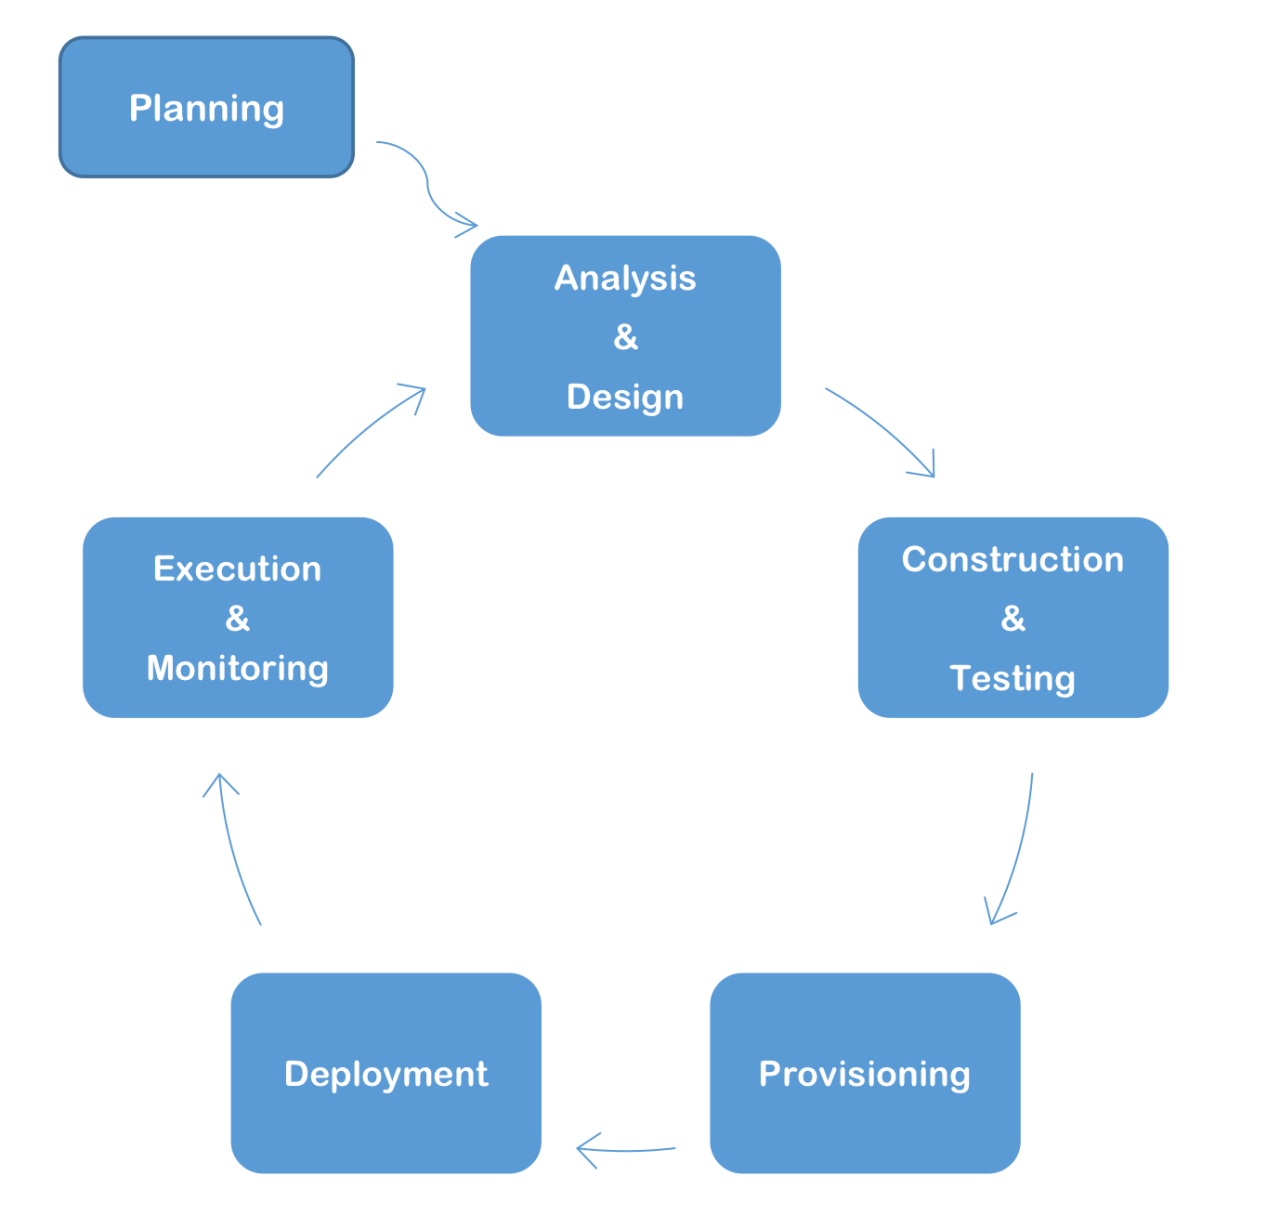
\includegraphics[width=0.5\textwidth]{./figure/PMZ/life} %插入图片,[]中设置图片大小,{}中是图片文件名
		\caption{Life circle of online study lounge system} %最终文档中希望显示的图片标题
		\label{life} %用于文内引用的标签

	\end{figure}
\begin{figure}[H]
		\centering %图片居中
		\includegraphics[width=0.5\textwidth]{./figure/PMZ/WSO} %插入图片,[]中设置图片大小,{}中是图片文件名
		\caption{Web Service Orchestration} %最终文档中希望显示的图片标题
		\label{wso} %用于文内引用的标签

	\end{figure}
\begin{figure}[H]
		\centering %图片居中
		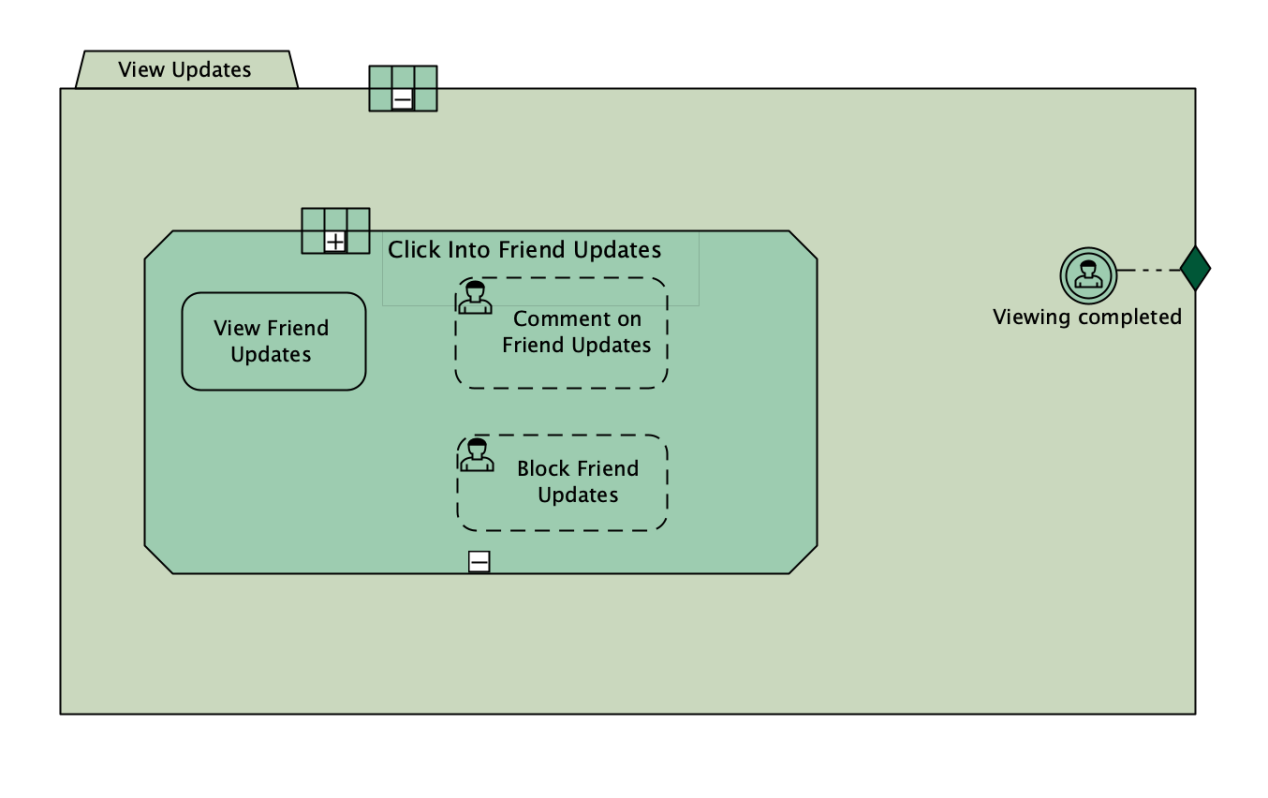
\includegraphics[width=1.0\textwidth]{./figure/PMZ/cmmn} %插入图片,[]中设置图片大小,{}中是图片文件名
		\caption{CMMN of Updates-viewing Service} %最终文档中希望显示的图片标题
		\label{cmmn} %用于文内引用的标签
	\end{figure}
In this CMMN of viewing updates, the user can click into friend's updates to view friend updates and give comment on this update or block this update so that the user will never see it again.
\\
Adjustment:
Changing all the inclusive gateways in BPMN of search-service and updates-issue service into exclusive gateways. Reason for adjustment: Because the tasks closely following these gateways can not execute at the same time.
\\
\begin{figure}[H]
		\centering %图片居中
		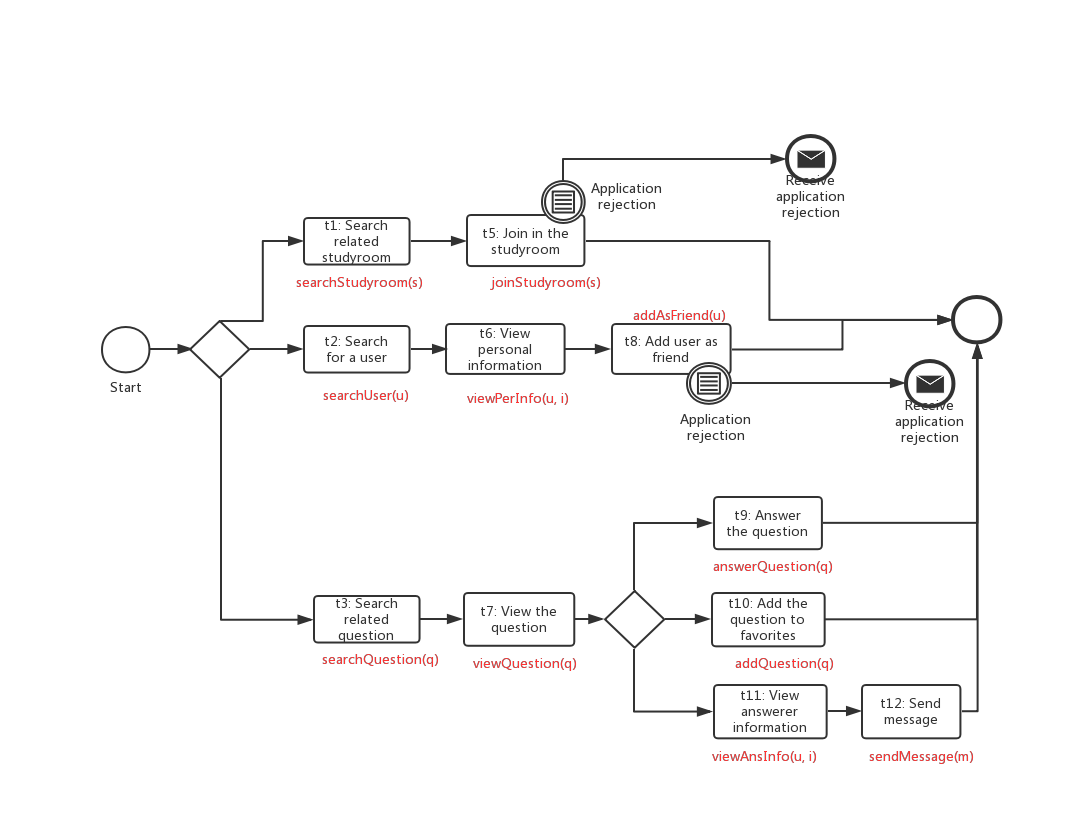
\includegraphics[width=1.0\textwidth]{./figure/PMZ/search} %插入图片,[]中设置图片大小,{}中是图片文件名
		\caption{Search Management} %最终文档中希望显示的图片标题
		\label{sea} %用于文内引用的标签
	\end{figure}
\begin{lstlisting}[language={XML}]
<bpmn:process id="Process_2" isExecutable="true">
	<bpmn:startEvent id="StartEvent">
        <bpmn:outgoing>SequenceFlow_1</bpmn:outgoing>
    </bpmn:startEvent>
    <bpmn:sequenceFlow id="SequenceFlow_1" sourceRef="StartEvent" targetRef="exclusiveGateway_1" />
    <bpmn:exclusiveGateway id="exclusiveGateway_1">
        <bpmn:incoming>SequenceFlow_1</bpmn:incoming>
        <bpmn:outgoing>SequenceFlow_2</bpmn:outgoing>
        <bpmn:outgoing>SequenceFlow_3</bpmn:outgoing>
        <bpmn:outgoing>SequenceFlow_4</bpmn:outgoing>
    </bpmn:exclusiveGateway>
    <bpmn:sequenceFlow id="SequenceFlow_2" sourceRef="exclusiveGateway_1" targetRef="Task_1" />
    <bpmn:sequenceFlow id="SequenceFlow_3" sourceRef="exclusiveGateway_1" targetRef="Task_2" />
    <bpmn:sequenceFlow id="SequenceFlow_4" sourceRef="exclusiveGateway_1" targetRef="Task_3" />
    <bpmn:task id="Task_1" name="Search related studyroom">
        <bpmn:incoming>SequenceFlow_2</bpmn:incoming>
        <bpmn:outgoing>SequenceFlow_5</bpmn:outgoing>
    </bpmn:task>
    <bpmn:task id="Task_2" name="Search for a user">
        <bpmn:incoming>SequenceFlow_3</bpmn:incoming>
        <bpmn:outgoing>SequenceFlow_6</bpmn:outgoing>
    </bpmn:task>
    <bpmn:task id="Task_3" name="Search related question">
        <bpmn:incoming>SequenceFlow_4</bpmn:incoming>
        <bpmn:outgoing>SequenceFlow_7</bpmn:outgoing>
    </bpmn:task>
    <bpmn:sequenceFlow id="SequenceFlow_5" sourceRef="Task_1" targetRef="Task_4" />
    <bpmn:sequenceFlow id="SequenceFlow_6" sourceRef="Task_2" targetRef="Task_5" />
    <bpmn:sequenceFlow id="SequenceFlow_7" sourceRef="Task_3" targetRef="Task_5" />
    <bpmn:task id="Task_4" name="Join in the studyroom">
        <bpmn:incoming>SequenceFlow_5</bpmn:incoming>
        <bpmn:outgoing>SequenceFlow_9</bpmn:outgoing>
    </bpmn:task>
    <bpmn:task id="Task_5" name="View personal information">
        <bpmn:incoming>SequenceFlow_6</bpmn:incoming>
        <bpmn:outgoing>SequenceFlow_10</bpmn:outgoing>
    </bpmn:task>
    <bpmn:task id="Task_6" name="View the question">
        <bpmn:incoming>SequenceFlow_7</bpmn:incoming>
        <bpmn:outgoing>SequenceFlow_11</bpmn:outgoing>
    </bpmn:task>
    <bpmn:sequenceFlow id="SequenceFlow_9" sourceRef="Task_4" targetRef="EndEvent_3" />
    <bpmn:sequenceFlow id="SequenceFlow_10" sourceRef="Task_5" targetRef="Task_7" />
    <bpmn:sequenceFlow id="SequenceFlow_11" sourceRef="Task_6" targetRef="exclusiveGateway_2" />
    <bpmn:boundaryEvent id="BoundaryEvent_1" name="Invitation rejection" attachedToRef="Task_4">
        <bpmn:outgoing>SequenceFlow_8</bpmn:outgoing>
        <bpmn:conditionalEventDefinition />
    </bpmn:boundaryEvent>
    <bpmn:sequenceFlow id="SequenceFlow_8" sourceRef="BoundaryEvent_1" targetRef="EndEvent_1" />
    <bpmn:endEvent id="EndEvent_1" name="Receive invitation rejection">
        <bpmn:ingoing>SequenceFlow_8</bpmn:ingoing>
        <bpmn:messageEventDefinition/>
    </bpmn:endEvent>
    <bpmn:sequenceFlow id="SequenceFlow_12" sourceRef="exclusiveGateway_2" targetRef="Task_8" />
    <bpmn:sequenceFlow id="SequenceFlow_13" sourceRef="exclusiveGateway_2" targetRef="Task_9" />
    <bpmn:sequenceFlow id="SequenceFlow_14" sourceRef="exclusiveGateway_2" targetRef="Task_10" />
    <bpmn:sequenceFlow id="SequenceFlow_15" sourceRef="Task_7" targetRef="EndEvent_3" />
    <bpmn:task id="Task_7" name="Add user as friend">
        <bpmn:incoming>SequenceFlow_10</bpmn:incoming>
        <bpmn:outgoing>SequenceFlow_15</bpmn:outgoing>
    </bpmn:task>
    <bpmn:task id="Task_8" name="Answer the question">
        <bpmn:incoming>SequenceFlow_12</bpmn:incoming>
        <bpmn:outgoing>SequenceFlow_17</bpmn:outgoing>
    </bpmn:task>
    <bpmn:task id="Task_9" name="Add the question to favorites">
        <bpmn:incoming>SequenceFlow_13</bpmn:incoming>
        <bpmn:outgoing>SequenceFlow_18</bpmn:outgoing>
    </bpmn:task>
    <bpmn:task id="Task_10" name="View answerer's information">
        <bpmn:incoming>SequenceFlow_14</bpmn:incoming>
        <bpmn:outgoing>SequenceFlow_19</bpmn:outgoing>
    </bpmn:task>
    <bpmn:boundaryEvent id="BoundaryEvent_2" name="Invitation rejection" attachedToRef="Task_7">
        <bpmn:outgoing>SequenceFlow_16</bpmn:outgoing>
        <bpmn:conditionalEventDefinition />
    </bpmn:boundaryEvent>
    <bpmn:sequenceFlow id="SequenceFlow_16" sourceRef="BoundaryEvent_2" targetRef="EndEvent_2" />
    <bpmn:endEvent id="EndEvent_2" name="Receive invitation rejection">
        <bpmn:ingoing>SequenceFlow_16</bpmn:ingoing>
        <bpmn:messageEventDefinition/>
    </bpmn:endEvent>
    <bpmn:sequenceFlow id="SequenceFlow_17" sourceRef="Task_8" targetRef="EndEvent_3" />
    <bpmn:sequenceFlow id="SequenceFlow_18" sourceRef="Task_9" targetRef="EndEvent_3" />
    <bpmn:sequenceFlow id="SequenceFlow_19" sourceRef="Task_10" targetRef="Task_11" />
    <bpmn:task id="Task_11" name="Send message">
        <bpmn:incoming>SequenceFlow_14</bpmn:incoming>
        <bpmn:outgoing>SequenceFlow_20</bpmn:outgoing>
    </bpmn:task>
    <bpmn:sequenceFlow id="SequenceFlow_20" sourceRef="Task_11" targetRef="EndEvent_3" />
    <bpmn:endEvent id="EndEvent_3">
        <bpmn:ingoing>SequenceFlow_9</bpmn:outgoing>
        <bpmn:ingoing>SequenceFlow_15</bpmn:outgoing>
        <bpmn:ingoing>SequenceFlow_17</bpmn:outgoing>
        <bpmn:ingoing>SequenceFlow_18</bpmn:outgoing>
        <bpmn:ingoing>SequenceFlow_20</bpmn:outgoing>
    </bpmn:endEvent>
</bpmn:process>
\end{lstlisting}
\begin{figure}[H]
		\centering %图片居中
		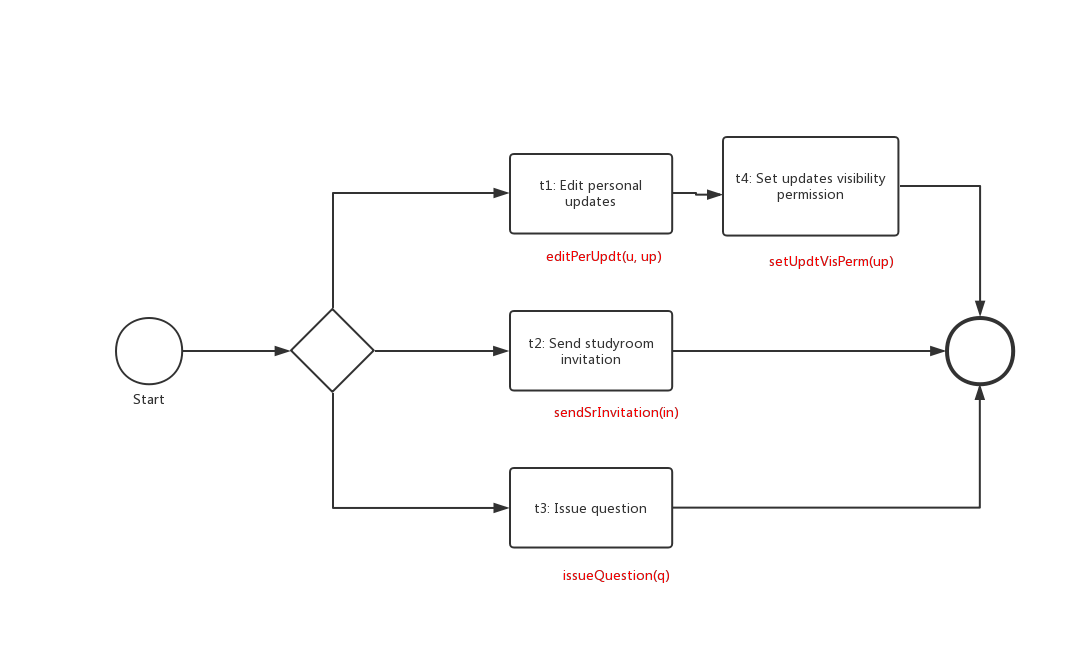
\includegraphics[width=1.0\textwidth]{./figure/PMZ/update} %插入图片,[]中设置图片大小,{}中是图片文件名
		\caption{Updates Issue Management} %最终文档中希望显示的图片标题
		\label{up} %用于文内引用的标签
	\end{figure}
\begin{lstlisting}[language={XML}]]
<bpmn:process id="Process_3" isExecutable="true">
	<bpmn:startEvent id="StartEvent">
        <bpmn:outgoing>SequenceFlow_1</bpmn:outgoing>
    </bpmn:startEvent>
    <bpmn:sequenceFlow id="SequenceFlow_1" sourceRef="StartEvent" targetRef="exclusiveGateway" />
    <bpmn:exclusiveGateway id="exclusiveGateway">
        <bpmn:incoming>SequenceFlow_1</bpmn:incoming>
        <bpmn:outgoing>SequenceFlow_2</bpmn:outgoing>
        <bpmn:outgoing>SequenceFlow_3</bpmn:outgoing>
        <bpmn:outgoing>SequenceFlow_4</bpmn:outgoing>
    </bpmn:exclusiveGateway>
    <bpmn:sequenceFlow id="SequenceFlow_2" sourceRef="exclusiveGateway" targetRef="Task_1" />
    <bpmn:sequenceFlow id="SequenceFlow_3" sourceRef="exclusiveGateway" targetRef="Task_2" />
    <bpmn:sequenceFlow id="SequenceFlow_4" sourceRef="exclusiveGateway" targetRef="Task_3" />
    <bpmn:task id="Task_1" name="Edit Personal updates">
    	<bpmn:ingoing>SequenceFlow_2</bpmn:ingoing>
    	<bpmn:outgoing>SequenceFlow_5</bpmn:outgoing>
    </bpmn:task>
    <bpmn:task id="Task_2" name="Send studyroom invitation">
    	<bpmn:ingoing>SequenceFlow_3</bpmn:ingoing>
    	<bpmn:outgoing>SequenceFlow_6</bpmn:outgoing>
    </bpmn:task>
    <bpmn:task id="Task_3" name="Issue question">
    	<bpmn:ingoing>SequenceFlow_4</bpmn:ingoing>
    	<bpmn:outgoing>SequenceFlow_7</bpmn:outgoing>
    </bpmn:task>
    <bpmn:sequenceFlow id="SequenceFlow_5" sourceRef="Task_1" targetRef="Task_4" />
    <bpmn:sequenceFlow id="SequenceFlow_6" sourceRef="Task_2" targetRef="EndEvent" />
    <bpmn:sequenceFlow id="SequenceFlow_7" sourceRef="Task_3" targetRef="EndEvent" />
    <bpmn:task id="Task_4" name="Set updates visibility permission">
    	<bpmn:ingoing>SequenceFlow_5</bpmn:ingoing>
    	<bpmn:outgoing>EndEvent</bpmn:outgoing>
    </bpmn:task>
    <bpmn:sequenceFlow id="SequenceFlow_8" sourceRef="Task_4" targetRef="EndEvent" />
    <bpmn:endEvent id="StartEvent">
        <bpmn:ingoing>SequenceFlow_6</bpmn:ingoing>
        <bpmn:ingoing>SequenceFlow_7</bpmn:ingoing>
        <bpmn:ingoing>SequenceFlow_8</bpmn:ingoing>
    </bpmn:endEvent>
</bpmn:process>
\end{lstlisting}

\subsubsection{Overall System architecture}
\noindent 
The overall system architecture is mainly composed of the presentation layer. core application layer, and SOA core competence layer. The unified user access is achieved through the portal. This module mainly includes user account information management and storage, user login identity authentication, and access request load balancing. The core application layer includes users, social, learning, Q\&A, and general business systems. The core competence layer of SOA consists of three parts: enterprise service bus, service management and registration library, and composite service operation engine. Among them, the Enterprise Service Bus (ESB) is a central component of the core competence layer of SOA. It is responsible for accessing various service resources. Through the use of a unified service interface, various services or applications and services can be easily accessed by each other. The structure replaces the original point-to-point structure between services, greatly optimizing the system connection architecture and reducing the complexity of system integration. The composite service operation engine usually runs on top of a standard process engine, such as the BPEL process engine.    

ESB Realize the functions of message passing, service routing, format conversion, transaction integrity guarantee, data analysis and processing, secure transmission, application adaptation, protocol conversion, etc.
\begin{figure}[H]
  \centering %图片居中
  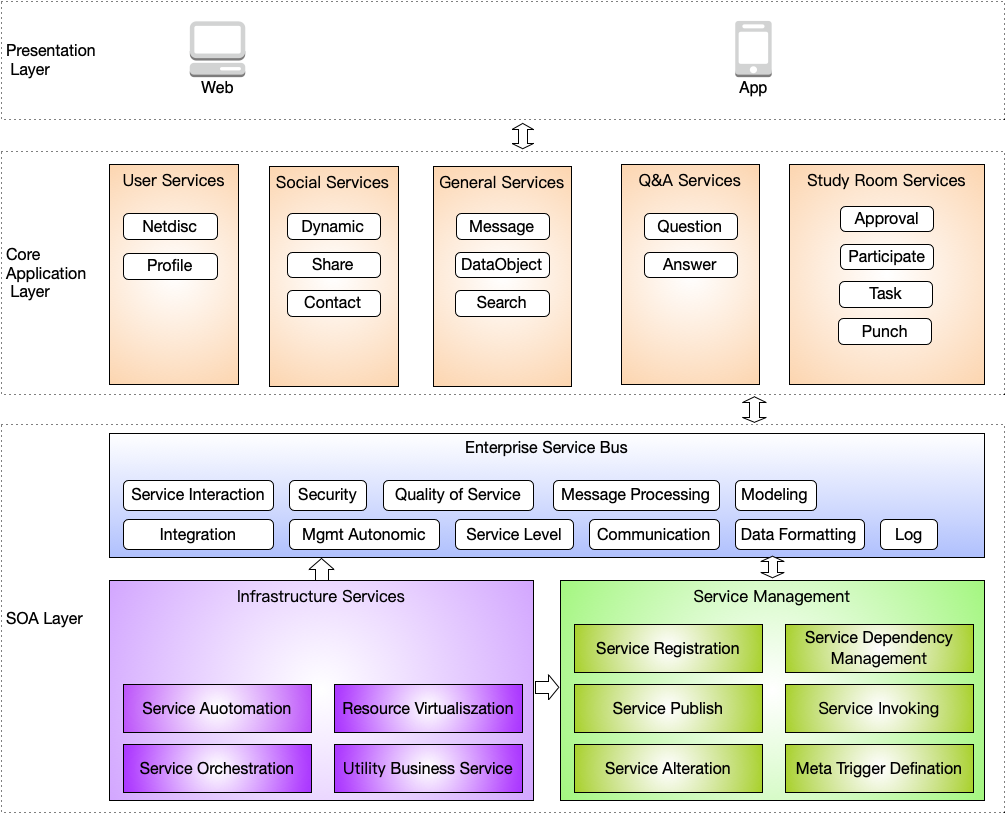
\includegraphics[width=1.0\textwidth]{figure/MWZH/odesb} %插入图片,[]中设置图片大小,{}中是图片文件名
  \caption{The Overall System Architecture} %最终文档中希望显示的图片标题
  \label{fig11}
\end{figure}

\subsubsection{Services Interaction}
Our design contain 5 modules, including 4 high-level functional module (User, Social, Study and Q\&A) and 1 supporting module(General). 

Functional module implement services with different functionalities. User Module contain profile edit service, login/register service, follow user service. Q\&A Module contain question add/edit/remove/follow and answer add/edit/remove/comment/vote service. Social module contains dynamic/contact add/edit/remove, block dynamic/contact, send/receive message, search contact service. Study module contains check/add/remove/edit calendar/task/studyroom/course, generate attendency/study report services. These services rely on basic services in General module. For instance, add calendar service instudy module will invoke the add object service in general module.



\begin{figure}[H]
    \centering %图片居中
    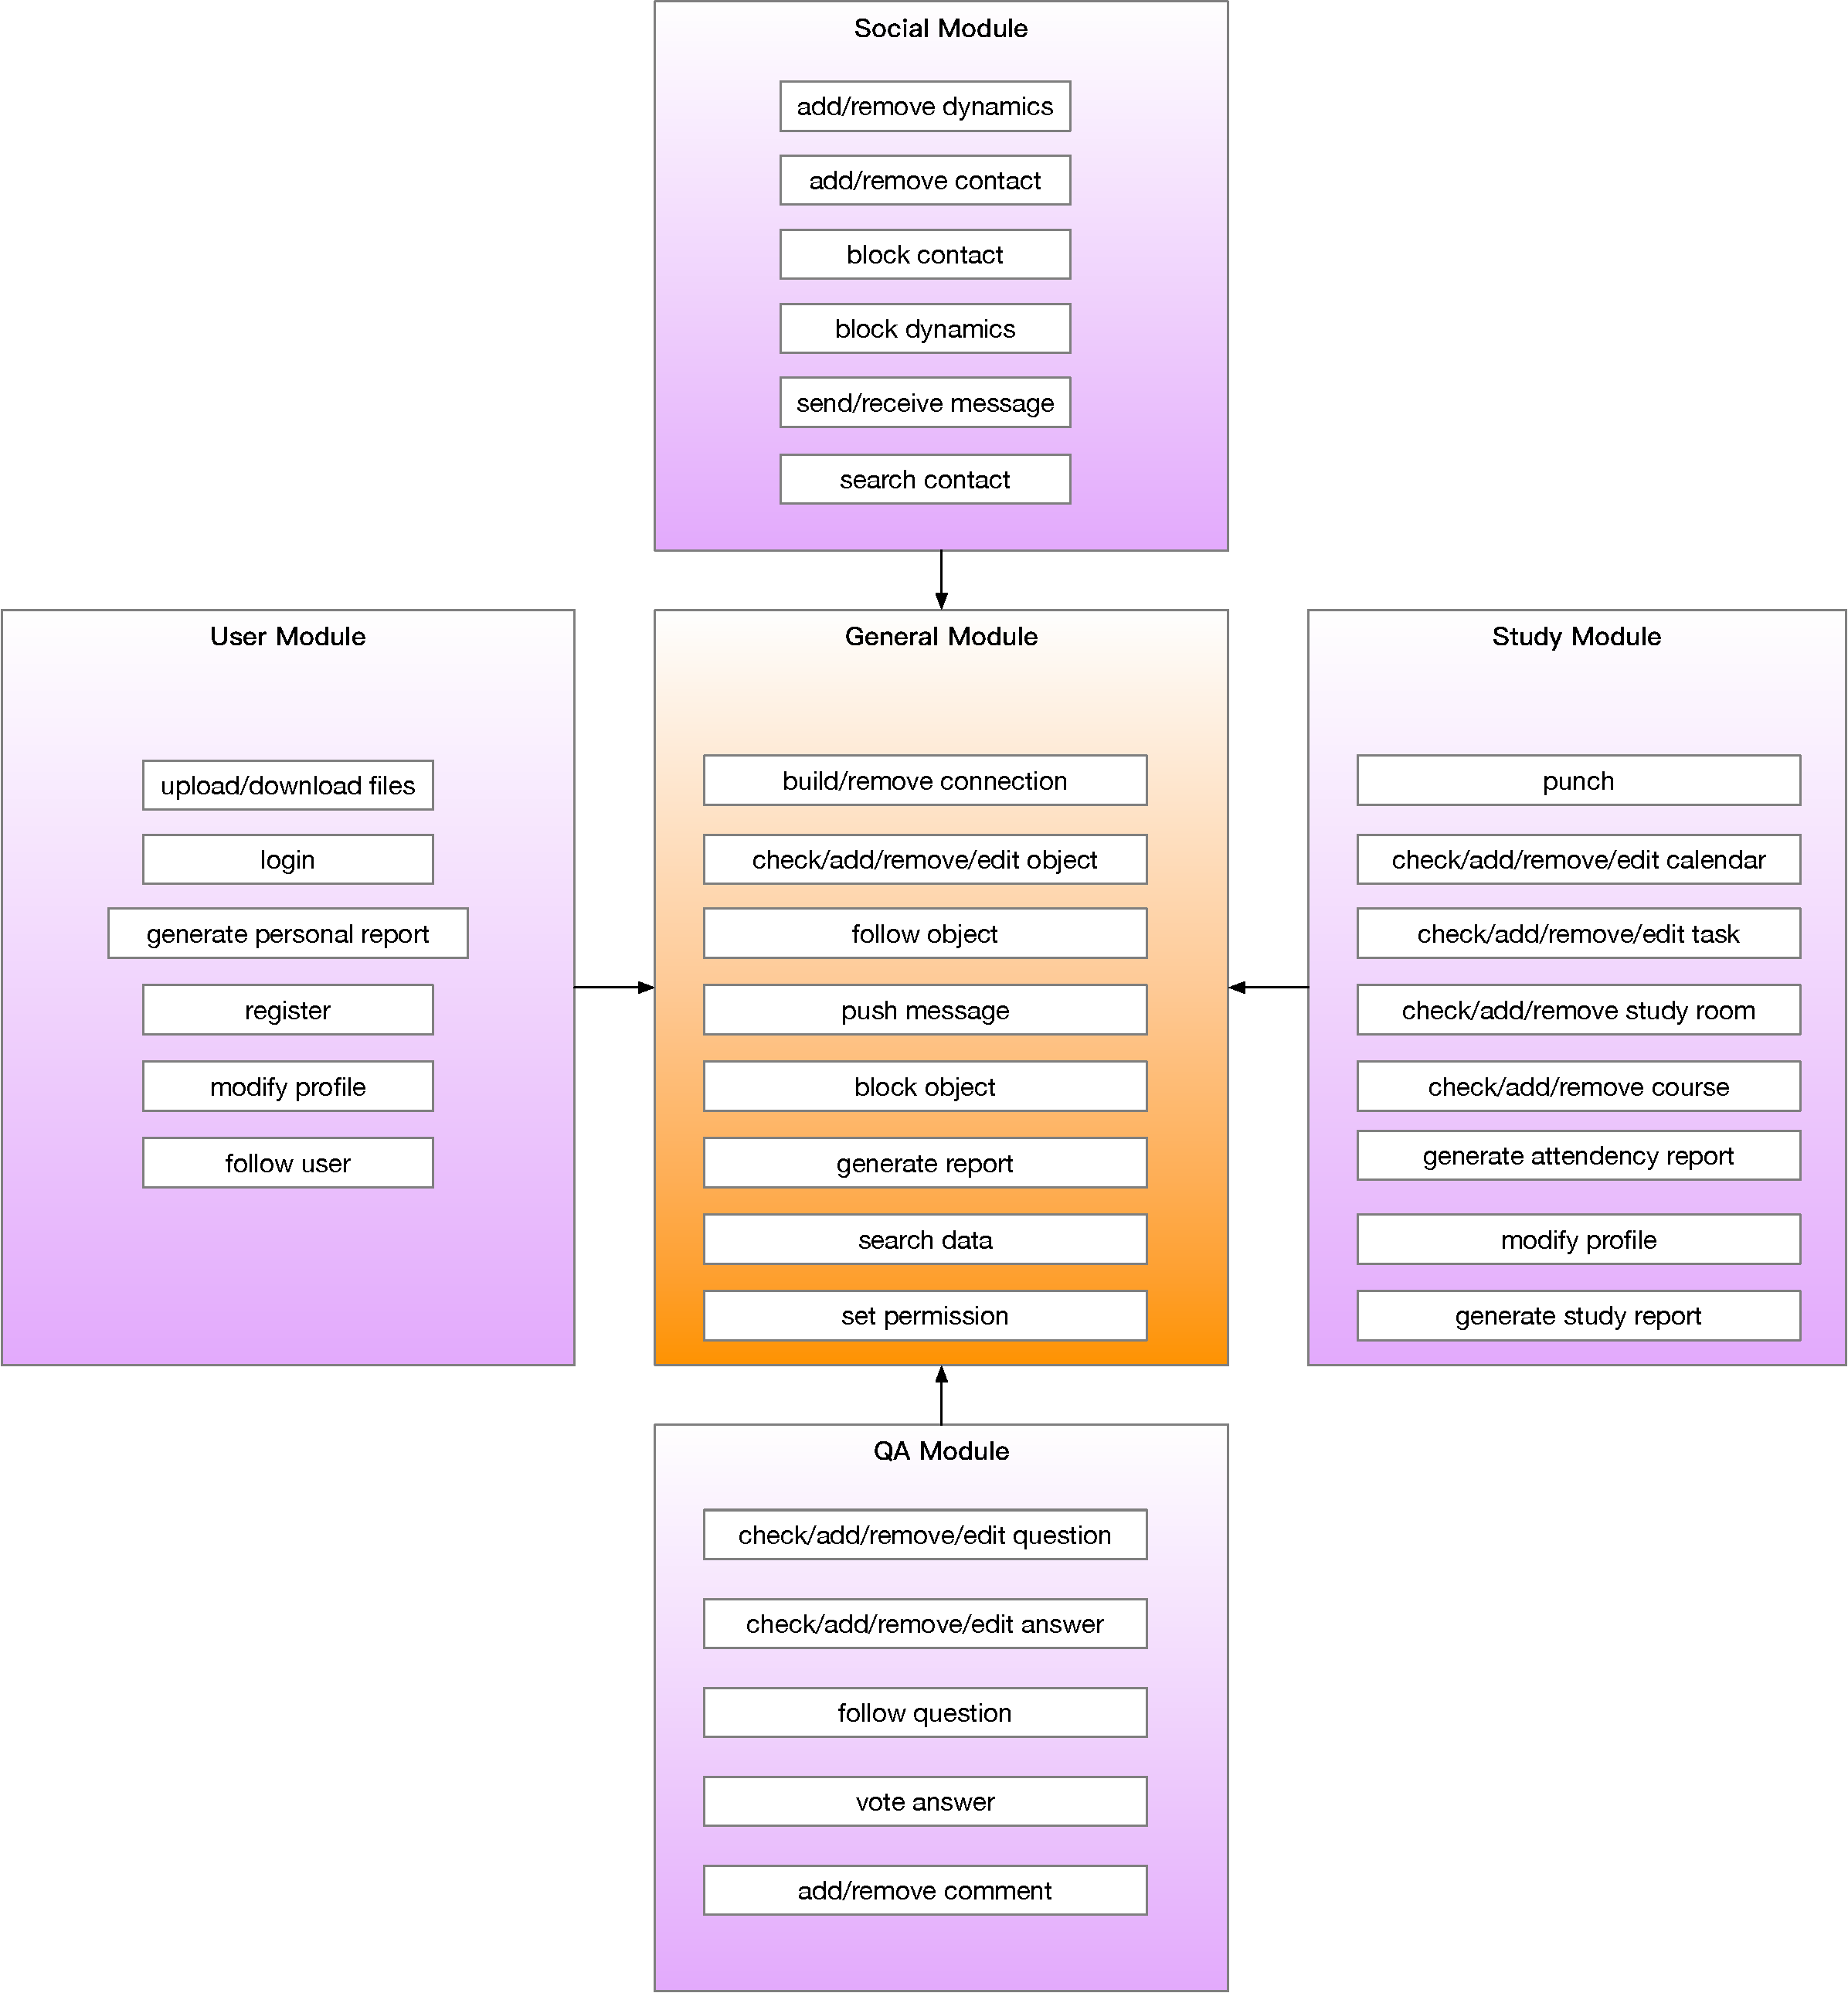
\includegraphics[width=1.0\textwidth]{figure/MWZH/services} %插入图片,[]中设置图片大小,{}中是图片文件名
    \caption{The services in different modules} %最终文档中希望显示的图片标题
    \label{fig12}
\end{figure}
\subsubsection{Service Publish/Interaction/Description}
We use UDDI for service publish and find. Web services descriptions contain four types of information:
\begin{itemize}
    \item Business information
    \item Service information
    \item Binding information
    \item Information about specifications of services
\end{itemize}
For main entities of the UDDI registry are described as :
\begin{itemize}
    \item businessEntity
    \item businessService
    \item bindingTemplate
    \item tModel
\end{itemize}
\begin{figure}[H]
    \centering %图片居中
    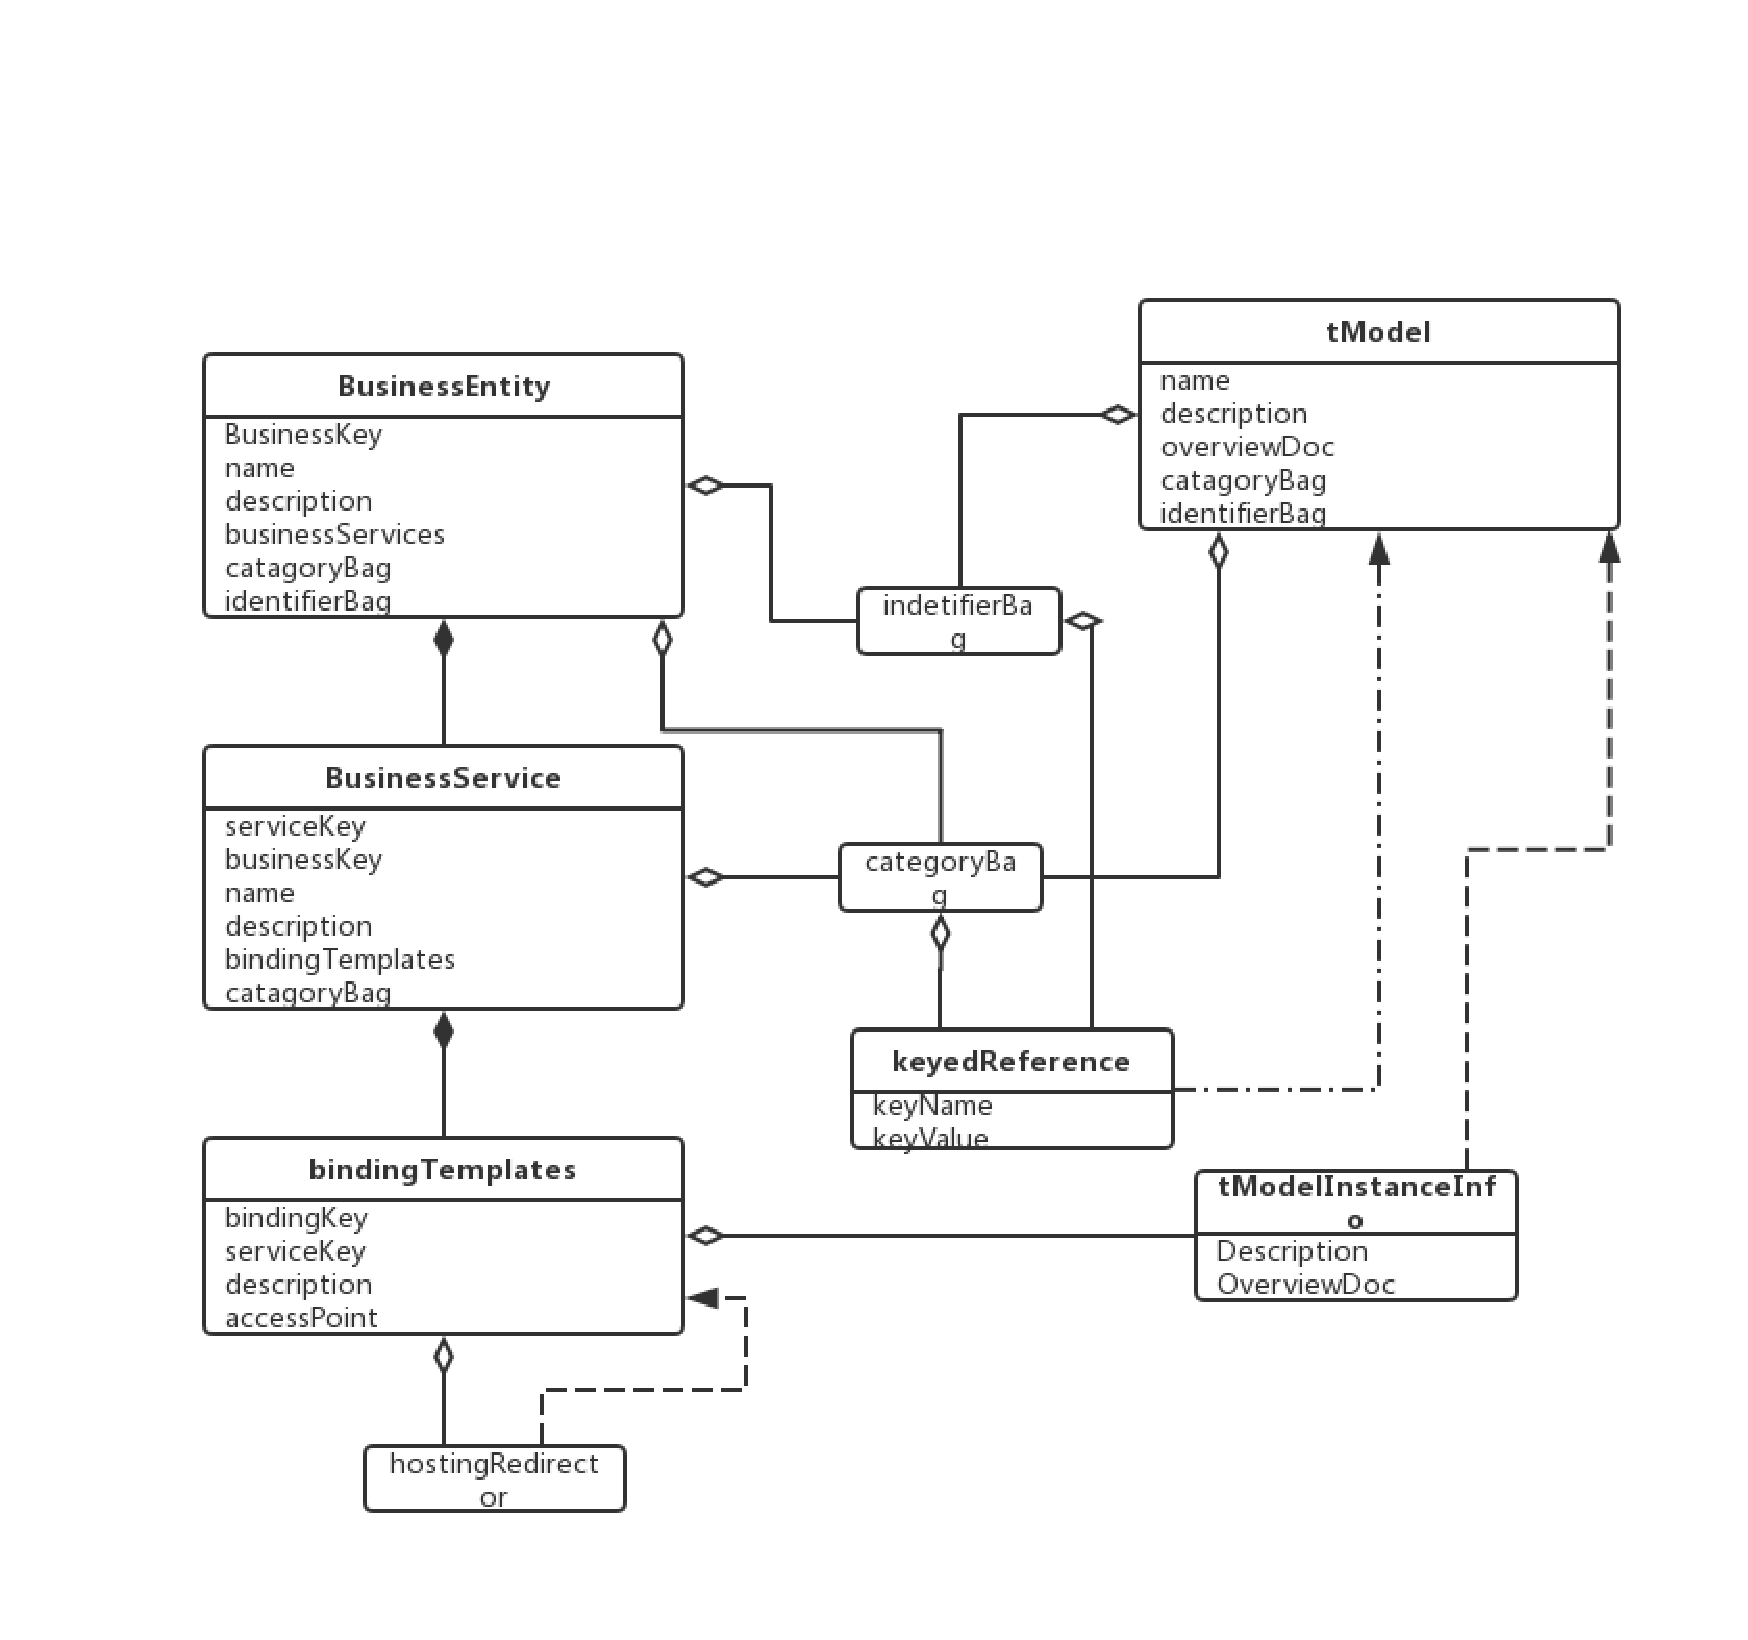
\includegraphics[width=1.0\textwidth]{./figure/MWZH/UDDIInformationModel} %插入图片,[]中设置图片大小,{}中是图片文件名
    \caption{UDDI} %最终文档中希望显示的图片标题
    \label{wsc} %用于文内引用的标签
\end{figure}

\subsubsection{Service Description}
We use WSDL to describe our service detail.
for example comment service WSDL file are like:
\begin{lstlisting}[language={XML}]
    <?xml version="1.0"?>
<definitions name="Vote"
             targetNamespace="http://csci927.com/vote.wsdl"
             xmlns:tns="http://csci927.com/vote.wsdl"
             xmlns:xsd1="http://csci927.com/vote.xsd"
             xmlns:soap="http://schemas.xmlsoap.org/wsdl/soap/"
             xmlns="http://schemas.xmlsoap.org/wsdl/">
              
  
  <types>
    <schema targetNamespace="http://csci927.com/vote.xsd"
            xmlns="http://www.w3.org/1999/XMLSchema">
      <element name="VoteRequest">
        <complexType>
          <all>
            <element name="SessionId" type="string"/>
            <element name="AnswerId" type="string"/>
            <element name="VoteType" type="int"/>
          </all>
        </complexType>
      </element>
      <element name="VoteResult">
        <complexType>
          <all>
            <element name="ReturnCode" type="int"/>
            <element name="ReturnMessage" type="string"/>
          </all>
        </complexType>
      </element>
    </schema>
  </types>
  <message name="VoteInput">
    <part name="body" element="xsd1:VoteRequest"/>
  </message>
  
  <message name="VoteOutput">
    <part name="body" element="xsd1:VoteResult"/>
  </message>

  <portType name="VotePortType">
    <operation name="Vote">
      <input message="tns:VoteInput"/>
      <output message="tns:VoteOutput"/>
    </operation>
  </portType>

  <binding name="VoteBinding" type="tns:VotePortType">
    <soap:binding style="document" transport="http://schemas.xmlsoap.org/soap/http">
      <operation name="Vote">
        <soap:operation soapAction="http://csci927.com/vote">
          <input>
            <soap:body use="literal" namespace="http://csci927.com/vote.xsd"
                       encodingStyle="http://schemas.xmlsoap.org/soap/encoding/"/>
          </input>
          <output>
            <soap:body use="literal" namespace="http://csci927.com/vote.xsd"
                       encodingStyle="http://schemas.xmlsoap.org/soap/encoding/"/>
          </output>
        </soap:operation>
      </operation>
    </soap:binding>
  </binding>

  <service name="VoteService">
    <documentation>Vote Account Service</documentation> 
    <port name="VotePort" binding="tns:VoteBinding">
    <soap:address location="http://csci927.com/vote"/>
    </port>
  </service>
  
</definitions>
\end{lstlisting}
And the relative SOAP pattern Request and Response are like this:

\begin{lstlisting}
    POST /StockQuote HTTP/1.1
    Host: example.com
    Content-Type: text/xml; charset="utf-8"
    Content-Length: nnnn
    SOAPAction: "http://example.com/Comment"
     
    <SOAP-ENV:Envelope xmlns:SOAP-ENV="http://schemas.xmlsoap.org/soap/envelope/"
                       SOAP-ENV:encodingStyle="http://schemas.xmlsoap.org/soap/encoding/">
      <SOAP-ENV:Body>
        <m:CommentRequest xmlns:m="http://example.com/comment.xsd">
          <SessionId>123nkdf1239jfasdkf123123#d</SessionId>
          <DataType>answer</DataType>
          <ObjectId>fsdhiuh1239hoewhf02uhfsdpr23</ObjectId>
          <Comment>The Answer is Good!~</Comment>
        </m:CommentRequest>
      </SOAP-ENV:Body>
    </SOAP-ENV:Envelope>


    HTTP/1.1 200 OK
    Content-Type: text/xml; charset="utf-8"
    Content-Length: nnnn
    
    <SOAP-ENV:Envelope xmlns:SOAP-ENV="http://schemas.xmlsoap.org/soap/envelope/"
                    SOAP-ENV:encodingStyle="http://schemas.xmlsoap.org/soap/encoding/"/>
    <SOAP-ENV:Body>
        <m:CommentResult xmlns:m=" http://example.com/comment.xsd ">
        <ReturnCode>0</ReturnCode>
        <ReturnMessage>Success</ReturnMessage>
        </m:CommentResult >
    </SOAP-ENV:Body>
    </SOAP-ENV:Envelope>

\end{lstlisting}

\subsubsection{SOA Structure}
We also draw the relationships between the core parts of a SOA
\begin{figure}[H]
  \centering %图片居中
  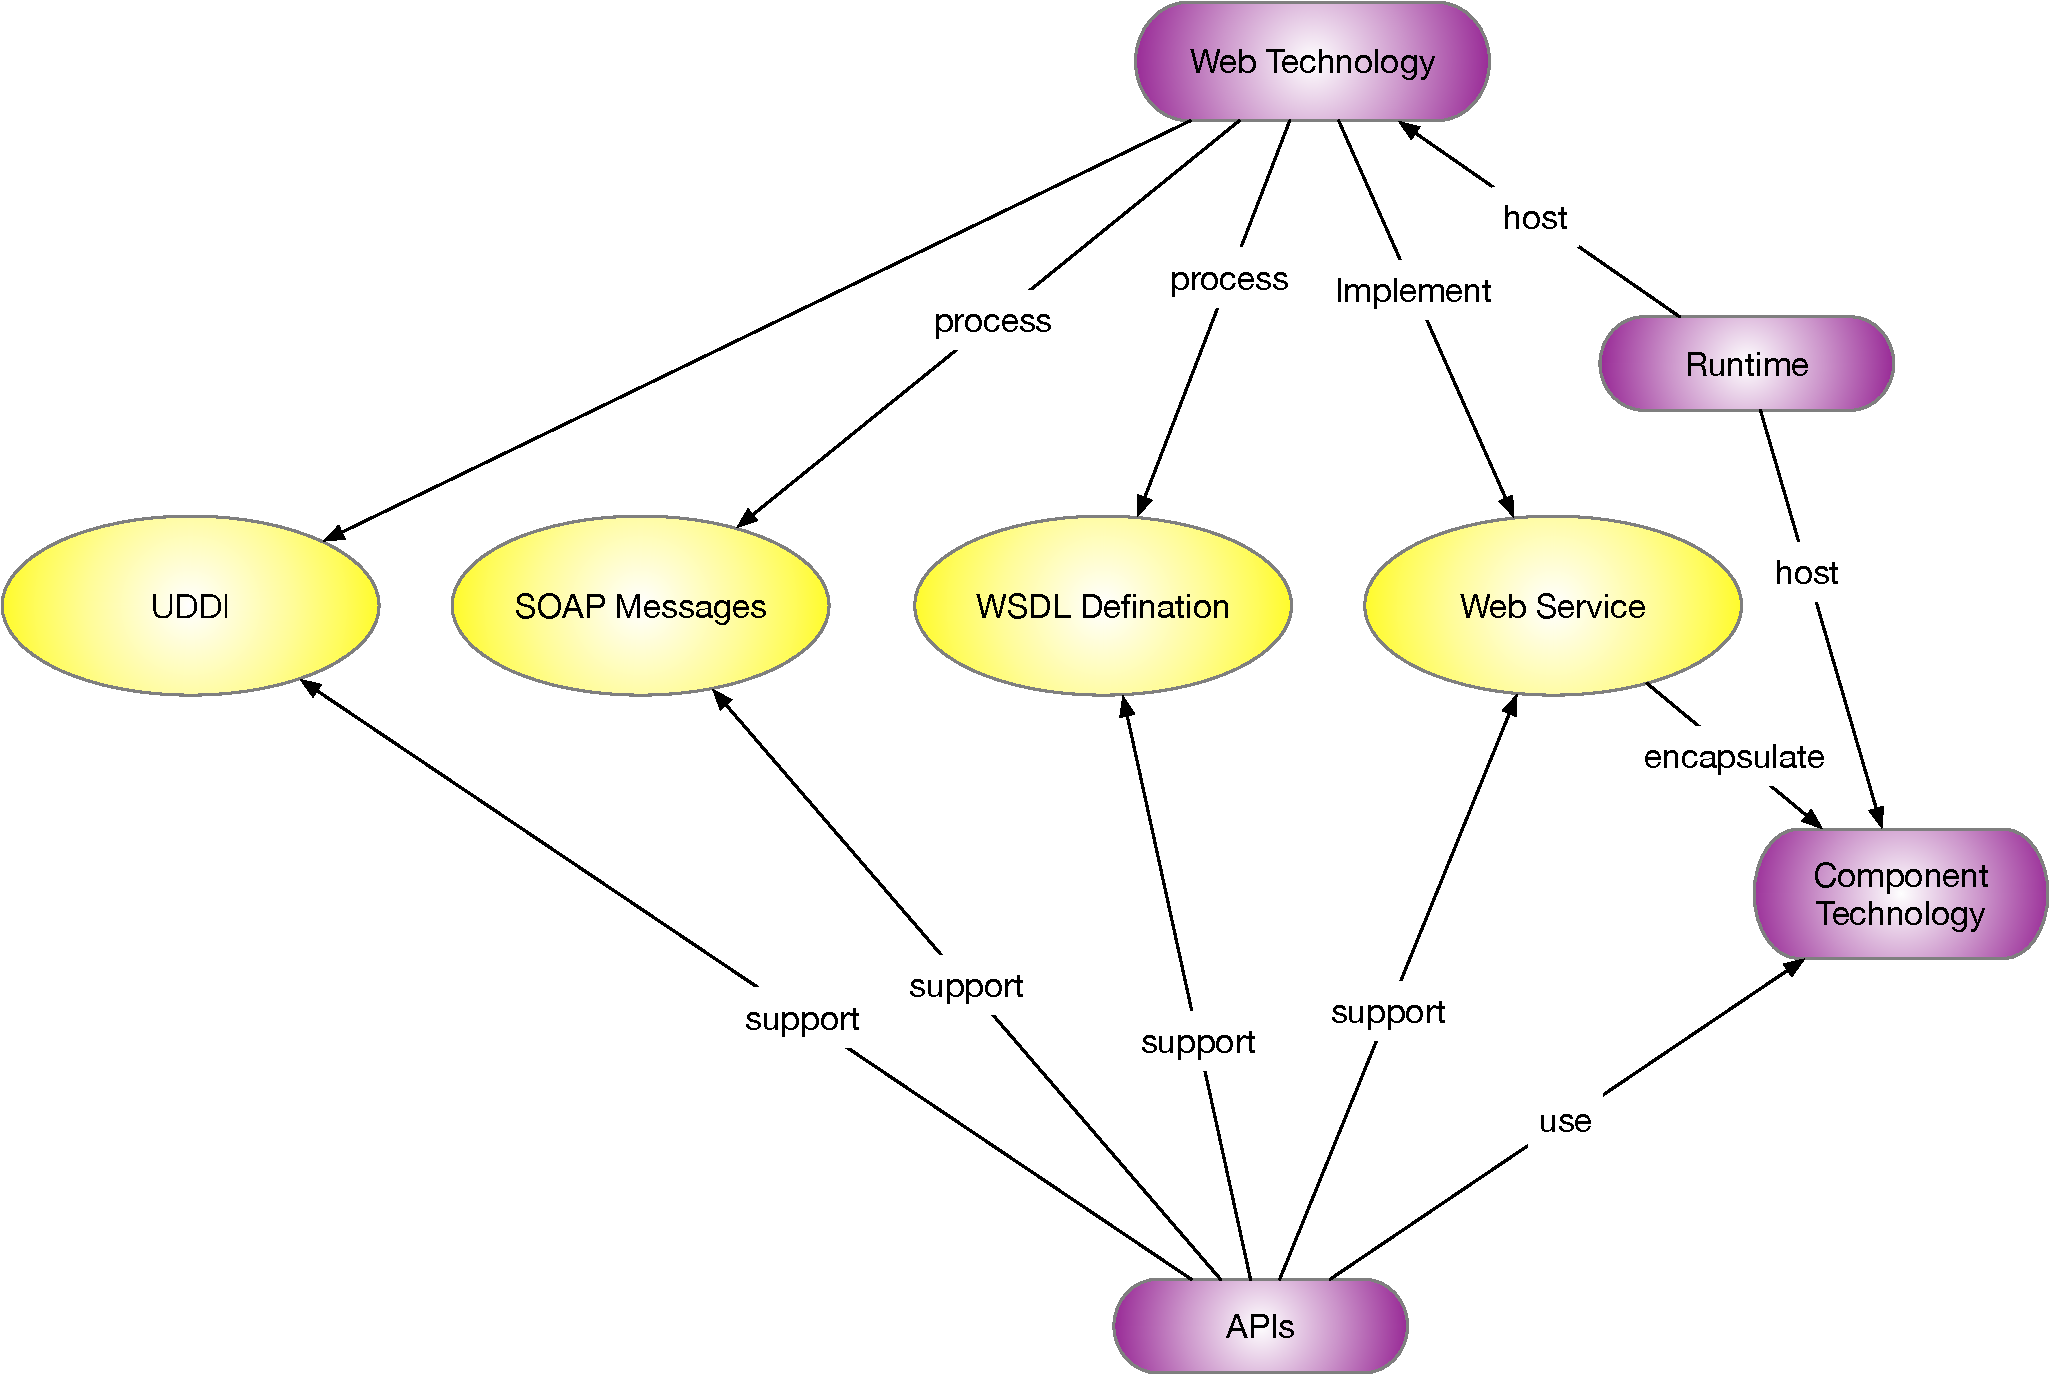
\includegraphics[width=1.0\textwidth]{./figure/MWZH/corepartssoa} %插入图片,[]中设置图片大小,{}中是图片文件名
  \caption{Relationships between the core parts of a SOA} %最终文档中希望显示的图片标题
  \label{wsc} %用于文内引用的标签
\end{figure}

% \subsubsection{Semantical Effect Annotation For QA Services}


\end{document}
